%% Springer Nature (sn-jnl, template v3.1 Dec 2024) version of the EngageNet engagement paper.
%% Target (since 2026-10-16): Journal of Ambient Intelligence and Humanized Computing (journal 12652), whose
%% guidelines require \documentclass[iicol,sn-basic]{sn-jnl} (two columns, author-year references), abstract
%% 150-250 words, 4-6 keywords, decimal headings with at most three levels, "Statements and Declarations" before
%% the references, LLM use documented in the Methods, references alphabetized with full DOI links, no reduced
%% fonts in tables or figures. The 12-page limit is NOT applied to this version (Yuvraj, 2026-10-16); the earlier
%% MTAP target (Track 5) used the same file with [Numbered] citations.
%% Section pattern follows the two Springer exemplars chosen by Yuvraj (J Ambient Intell Humaniz Comput
%% 17:1579-1598, 2026; J Signal Process Syst 97:269-280, 2025); prose follows the FoleyGAN style (Ghose & Prevost,
%% IEEE TMM 2023). Numbers trace to results/fullclip/ and results/paper_springer/ (scripts/paper/*.py), except
%% the training sweep and the 12-of-13 audio check (results/night/, docs/plan.md Sec. 13.14), the 67.82 threshold
%% oracle (Sec. 19.6), the equal-thirds and validation-selected fusions (Sec. 19.7.1) and the OpenFace timing
%% (Sec. 18.16). Numbers re-checked against these sources on 2026-10-07. Section 4 re-checked 2026-10-16: the three
%% pre-training stages trace to results/engagenet_h8_uniform_fullaudio_v96 (CE, 1e-2, 30 ep), results/v12_05_* (ordinal,
%% 1e-4, 25 ep) and results/exp2026/E04_* (ordinal, 5e-5, 8 ep); v12_03 is not in the lineage. [iicol] = two-column layout
%% (user manual Sec. 2.1; add [referee] for double spacing); full-width tables/figures use table*/figure* (manual Sec. 7.3).
%% Draft note: the template asks for one .tex file; before submission replace each \input{figures/...}
%% by the compiled figure PDF (Fig1.pdf ...) and paste the .bbl into this file.

\documentclass[pdflatex,iicol,sn-basic]{sn-jnl}

\usepackage{graphicx}
\graphicspath{{figures/}}
\usepackage{multirow}
\usepackage{amsmath,amssymb,amsfonts}
\usepackage{xcolor}
\usepackage{booktabs}
\usepackage{algorithm}
\usepackage{algorithmicx}
\usepackage{algpseudocode}
\usepackage{tikz}
\usetikzlibrary{positioning,calc,decorations.pathreplacing}
\usepackage{pgfplots}
\pgfplotsset{compat=1.17}
% Shared figure colours (validated for colour-vision deficiency; see dataviz palette).
\definecolor{ours}{HTML}{2A78D6}      % our single models
\definecolor{fused}{HTML}{EB6834}     % our late fusion
\definecolor{published}{HTML}{8F8E88} % published EngageNet baselines
\definecolor{inkmuted}{HTML}{52514E}
\definecolor{boxfill}{HTML}{F3F2EF}
\definecolor{seqlo}{HTML}{FFFFFF}
\definecolor{seqhi}{HTML}{104281}


% Model name used throughout. Change it here only.
\newcommand{\ournet}{AVB-Engage}

\raggedbottom

\begin{document}

\title[Audio-visual and facial-behavior fusion for ordinal engagement recognition]{Audio-Visual Cross-Attention and Facial-Behavior Fusion for Ordinal Student Engagement Recognition in Online Learning}

% Author names withheld in this draft, as in research/paper/paper.tex. MTAP is single-blind: names,
% affiliations, the corresponding author's e-mail and ORCIDs are required at submission.
\author*[1]{\fnm{First} \sur{Author}}\email{first.author@example.edu}
\author[1]{\fnm{Second} \sur{Author}}
\author[1]{\fnm{Third} \sur{Author}}
\affil*[1]{\orgdiv{Department}, \orgname{Organization}, \orgaddress{\city{City}, \state{State}, \country{Country}}}

\abstract{Automatic engagement recognition estimates from a webcam recording how engaged a student is during online learning. Published results on EngageNet, the online-learning engagement dataset with the most participants, use visual input only, although the recordings also contain audio. In this paper, we present \ournet, which combines an audio-visual cross-attention network with two models built on segment statistics of OpenFace action units, gaze and head pose. The class probabilities of the three models are averaged and decoded through the expected engagement level with thresholds fitted on the validation split, so that the order of the four engagement levels is used at prediction time. We evaluated \ournet{} on the official EngageNet test split over three training seeds. Audio alone does not exceed the majority-class predictor, but adding it to video raises top-1 accuracy in seven of nine trained networks, by 0.74 points on average. On identical weights, decoding through the expected level adds 2.00 points over argmax decoding, and averaging the network with the two behavior models adds about four points more, because the models make different errors. The same behavior descriptors learned by a branch inside the network change no metric. \ournet{} reaches 70.29\% top-1 accuracy and a mean absolute error of 0.401 levels, whereas the best published EngageNet test accuracy is 67.61\%.}

\keywords{Student engagement recognition, Audio-visual fusion, Cross-attention, Facial action units, Ordinal classification, Online learning}

\maketitle

\section{Introduction}\label{sec:intro}

In a classroom, an instructor judges whether students are following a lesson from several cues at once: where a student looks, the student's facial expression and posture, and whether the student speaks or responds. In an online class the instructor sees each student only through a webcam tile, and with many students on screen these cues are easy to miss. Automatic engagement recognition addresses this problem by estimating the engagement level of each student from the recording \citep{qarbal2025review,mandia2023review}. A system of this kind can report to the instructor which students were disengaged during which part of a session.

EngageNet \citep{singh2023engagenet} is a public benchmark for this task. Its participants watched three short educational videos on a web platform with their own webcams, and every ten-second clip of a recording is labeled with one of four ordered levels, from \emph{not engaged} to \emph{highly engaged}. The baselines released with the dataset and the methods proposed since read only the visual stream \citep{singh2023engagenet,vedernikov2024tcct,abedi2024stgcn,vedernikov2026priornet,augusma2026vemd}; the dataset authors set the audio aside because of background noise and missing audio. Two properties of the labels make the task harder than its four classes suggest. The levels are ordered, so calling a highly engaged student \emph{not engaged} is a larger error than calling the student \emph{engaged}. The levels are also imbalanced: half of the test clips are \emph{highly engaged}, so a model that always predicts this level is already right half of the time.

In this paper, we propose a model called \ournet{} (audio, video and behavior) that predicts the engagement level of a ten-second clip from three sources of evidence: the face frames, the audio track, and per-frame facial-behavior descriptors (Fig.~\ref{fig:concept}). For the face frames and the audio track, we follow audio-visual emotion recognition, in which cross-attention lets each modality attend to the other \citep{venkatraman2025avtca}. For the facial-behavior descriptors, we follow the best EngageNet baseline, which reads OpenFace action units, gaze and head pose \citep{singh2023engagenet}. Since the levels are ordered, we also read the output of the model as a position on the engagement scale rather than as four unrelated classes.

\begin{figure*}[t]
\centering
\resizebox{0.78\textwidth}{!}{% Fig. 1 -- problem framing (Introduction). Shares are the EngageNet test split (n = 2,256);
% the error share is the audio-visual network pooled over its three seeds.
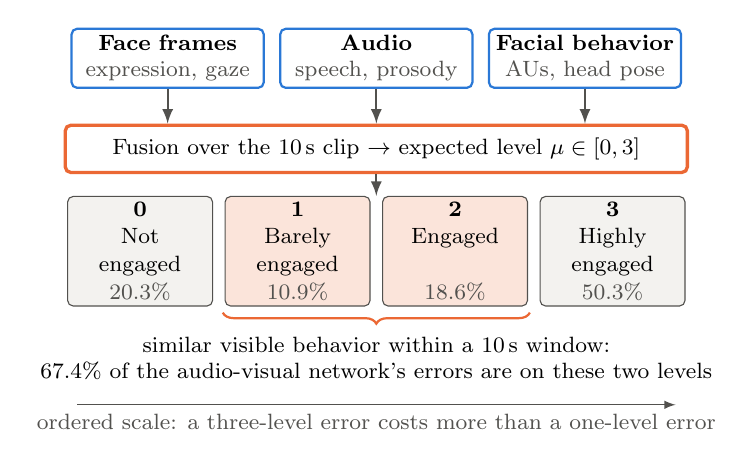
\begin{tikzpicture}[font=\footnotesize, >=latex,
  lvl/.style={draw=inkmuted, fill=boxfill, rounded corners=2pt, text width=1.7cm, minimum height=1.3cm, align=center, inner sep=2pt, execute at begin node={\setlength{\baselineskip}{10pt}\setlength{\lineskiplimit}{-10pt}}},
  cue/.style={draw=ours, thick, rounded corners=2pt, text width=2.3cm, minimum height=0.75cm, align=center, fill=white, inner sep=2pt}]
  \node[cue] (v) at (0.35,2.45) {\textbf{Face frames}\\\textcolor{inkmuted}{expression, gaze}};
  \node[cue] (a) at (3.0,2.45) {\textbf{Audio}\\\textcolor{inkmuted}{speech, prosody}};
  \node[cue] (b) at (5.65,2.45) {\textbf{Facial behavior}\\\textcolor{inkmuted}{AUs, head pose}};
  \node[draw=fused, very thick, rounded corners=2pt, minimum width=7.9cm, minimum height=0.6cm, fill=white] (m) at (3.0,1.3)
     {Fusion over the 10\,s clip $\rightarrow$ expected level $\mu\in[0,3]$};
  \foreach \s in {v,a,b} \draw[->, thick, inkmuted] (\s) -- (\s |- m.north);
  \node[lvl] (l0) at (0,0)   {\textbf{0}\\Not\\engaged\\\textcolor{inkmuted}{20.3\%}};
  \node[lvl, fill=fused!18] (l1) at (2.0,0) {\textbf{1}\\Barely\\engaged\\\textcolor{inkmuted}{10.9\%}};
  \node[lvl, fill=fused!18] (l2) at (4.0,0) {\textbf{2}\\Engaged\\\strut\\\textcolor{inkmuted}{18.6\%}};
  \node[lvl] (l3) at (6.0,0) {\textbf{3}\\Highly\\engaged\\\textcolor{inkmuted}{50.3\%}};
  \draw[->, thick, inkmuted] (m.south) -- (m.south |- l1.north);
  \draw[decorate, decoration={brace, amplitude=4pt, mirror}, fused, thick] (1.05,-0.78) -- (4.95,-0.78)
     node[midway, below=5pt, text=black, align=center]{similar visible behavior within a 10\,s window:\\ 67.4\% of the audio-visual network's errors are on these two levels};
  \draw[->, inkmuted] (-0.8,-1.95) -- node[below, text=inkmuted]{ordered scale: a three-level error costs more than a one-level error} (6.8,-1.95);
\end{tikzpicture}
}
\caption{Problem description. Face, audio and facial-behavior evidence from a 10\,s clip is fused into an expected level on the ordered four-level EngageNet scale. Percentages are the share of each level in the test split (2,256 clips). The two middle levels are both rare and visually similar; they receive 67.4\% of the errors of our audio-visual network (three seeds pooled)}
\label{fig:concept}
\end{figure*}

Fig.~\ref{fig:overview} shows the proposed model, which consists of three blocks. The first block (A) is an audio-visual network: an EfficientFace backbone \citep{zhao2021efficientface} encodes the face frames, a convolutional encoder encodes the log-mel spectrogram, and the two streams exchange information through three cross-attention stages before a linear layer predicts the probability of each level. The second block (B) contains two models that read the OpenFace descriptor of the same clip: a gradient-boosting classifier and a small Transformer encoder. Both read the descriptor as segment statistics, that is, the mean and standard deviation of each feature within each of 20 equal time segments. The third block (C) averages the three probability vectors and computes the expected level, the probability-weighted mean of the level indices, which three thresholds fitted on the validation split cut into the predicted level.

\begin{figure*}[t]
\centering
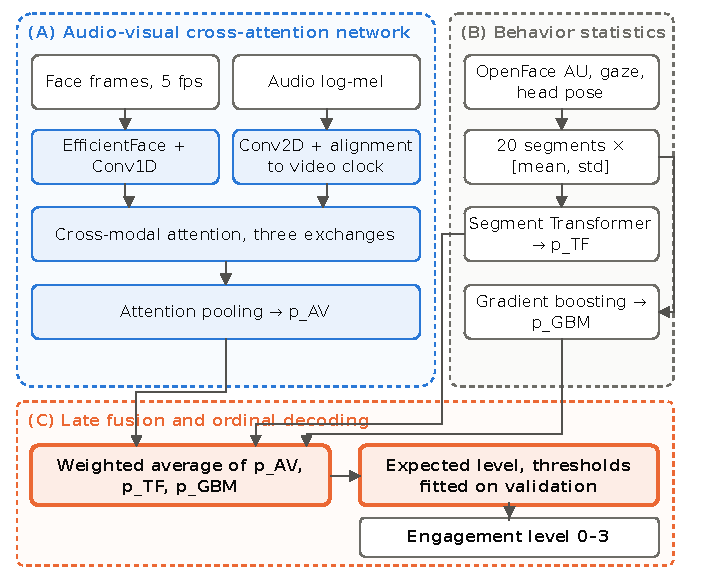
\includegraphics[width=0.85\textwidth]{overview}
\caption{Overview of \ournet. (A) The audio-visual network produces class probabilities $p_{\mathrm{AV}}$ from face frames and audio; (B) two models on segment statistics of the OpenFace descriptor produce $p_{\mathrm{TF}}$ and $p_{\mathrm{GBM}}$; (C) the three vectors are averaged and decoded into one of four ordered levels}
\label{fig:overview}
\end{figure*}

We chose these components for the following reasons. EfficientFace was trained for facial expression recognition, so the visual encoder starts from a face-specific representation rather than from generic image features. The audio encoder produces about twice as many time steps as there are video frames, so we pool the audio steps of each clip onto its video frames before the first exchange, which gives each visual token one audio token for the same time span. The segment statistics follow the tokenization of the best EngageNet baseline \citep{singh2023engagenet}, which makes the behavior models directly comparable with it. Finally, we keep the behavior models separate from the network and combine them only at the probability level, because models trained on different inputs with different learners can be expected to make different errors; Section~\ref{sec:results} tests this expectation.

The main contributions of this paper are as follows:
\begin{enumerate}
\item We present, to our knowledge, the first audio-visual evaluation on EngageNet. Audio alone does not exceed the majority-class predictor on this dataset, yet adding it to video raises top-1 accuracy in most of the trained networks we tested.
\item We measure, on identical trained weights, how much the decoding rule changes accuracy on the ordered engagement scale. Decoding through the expected level changes top-1 accuracy more than any training change we tested.
\item We show that facial-behavior descriptors help when they are summarized by segment statistics in separate models and averaged with the network, which exceeds the best published EngageNet test accuracy, and that the same descriptors learned inside the network change no metric. We trace the gain to the different errors of the three models.
\item We report top-1 accuracy, adjacent accuracy, mean absolute error and macro-F1 per seed and per level, five ablation studies, the computational cost of every component, and an analysis of where the remaining errors lie.
\end{enumerate}

The remainder of this paper is organized as follows. Section~\ref{sec:related} reviews related work. Section~\ref{sec:method} formulates the problem and describes the proposed model. Section~\ref{sec:exp} describes the dataset, the implementation details and the evaluation metrics. Section~\ref{sec:results} presents the results, the ablation studies, the computational cost, the error analysis and the limitations. Section~\ref{sec:conclusion} concludes the paper.

\section{Related work}\label{sec:related}

\subsection{Student engagement recognition}\label{sec:rw_engagement}

Engagement recognition asks a model to judge from a recording what an annotator judges from a learner's gaze, expression, posture and responses. Reviews cover the computer-vision methods for this task \citep{qarbal2025review}, its data and methods \citep{mandia2023review}, and the shallow and deep learners used for it \citep{theophilus2026review}. Two public datasets recur in this work. DAiSEE \citep{gupta2016daisee} labels webcam clips of 112 users for engagement, boredom, confusion and frustration, and CMOSE \citep{wu2024cmose} labels 12,193 segments of online presentation classes with 102 participants and provides audio as well as video. The methods differ mainly in what they read from the video. One group learns from the frames, for example multitask EfficientNet affective computing \citep{thiruthuvanathan2024multitask}, a class-attention video transformer \citep{ai2024classattention}, MSC-Trans, which fuses user-selected visual feature groups over time with an encoder--decoder structure \citep{xie2025msctrans}, and ViBED-Net, which combines face-aware and scene-aware spatio-temporal cues \citep{gothwal2025vibednet}. A second group reads explicit cues such as head pose \citep{mo2024headpose}, facial cues \citep{gupta2023facialcues}, or several cues per student and per class \citep{pabba2023multicues}. In this group, gradient boosting on facial action units has been used to estimate the mental states of learners in an intelligent tutoring system \citep{wang2026shap}, and a study on two engagement datasets reports that a gradient-boosting model with action units reaches higher accuracy than the deep networks it trained \citep{das2025optimizing}. Other work combines several modalities in a real-time feedback framework for higher education \citep{zhao2026multimodal} or compares modalities for online education \citep{immadisetty2025multimodality}. The closest result to our use of audio comes from CMOSE: adding audio features to its visual features raises accuracy only slightly over all test segments, but clearly on the quarter of segments that contain speech \citep{wu2024cmose}. In our work, we use both a learned frame encoder and explicit OpenFace descriptors, and we add the audio track.

\subsection{Engagement recognition on EngageNet}\label{sec:rw_engagenet}

Results on EngageNet are reported on different splits, so a comparison must first check which split a number comes from. To our knowledge, the baselines released with the dataset \citep{singh2023engagenet} are the only published results on the official test split, whose labels are distributed with the dataset. They are an LSTM, a CNN-LSTM, a TCN and a Transformer on OpenFace gaze, head-pose and action-unit features, a Transformer on MARLIN video features \citep{cai2023marlin}, and a Transformer that fuses both; the best is the Transformer on OpenFace features. This Transformer cuts each clip into 20 equal segments and describes each segment by the mean and standard deviation of its features. For the same baseline model, validation accuracy is 1.5--5.2 points higher than test accuracy. The methods proposed since report validation accuracy: TCCT-Net, a two-stream network that reads only two head-pose rotation signals instead of the 98 features of the baselines \citep{vedernikov2024tcct}; an ordinal spatial-temporal graph network on facial landmarks \citep{abedi2024stgcn}; PriorNet, a prior-guided face-video model \citep{vedernikov2026priornet}; and VE-MD, a variational encoder with multiple decoders, which has an audio branch for other datasets but uses video only on EngageNet \citep{augusma2026vemd}. GLP-fusion \citep{qin2026glpfusion} evaluates on the data of the EmotiW 2023 engagement sub-challenge, which the EngageNet authors organized \citep{dhall2023emotiw}, on a split of its own; it fuses global facial features, facial key points and physiological signals, all estimated from the video. GAN-generated frames have been used to augment the two rare levels of EngageNet, which raises macro-F1 in most of the training configurations tested; the evaluation split is not stated \citep{yulius2025gan}. Vision-language models have also been used to refine noisy EngageNet labels \citep{vedernikov2025vlmnoise}. All of these methods read the visual stream only. In our work, we report results on the official test split, which makes them comparable with the six baselines, and we add the audio track.

\subsection{Audio-visual fusion and facial representations}\label{sec:rw_av}

Audio-visual fusion has been developed mainly for emotion recognition, where the voice and the face express the same affective state. AVT-CA \citep{venkatraman2025avtca} fuses audio and video features with transformer cross-attention, in which the audio features attend to the video features and the video features attend to the audio features. Attention bottlenecks restrict the exchange between modalities to a few shared tokens \citep{nagrani2021attention}, and early fusion with dense audio-visual interactions has been trained by masked modeling \citep{mo2024earlyfusion}. Face-and-speech emotion recognition has also been built from convolutional and LSTM networks \citep{taware2025mer}, depression has been recognized from audio, video and text \citep{lu2026dstc}, and audio-visual action recognition has encoded frames and log-mel spectrograms with one Swin Transformer and fused them pairwise by co-attention \citep{kim2024avaction}. A review of multimodal emotion recognition covers both the complete-modality and the missing-modality setting \citep{li2026mersurvey}; the second is common in online classes, where microphones are often muted. In emotion recognition the speaker's voice carries the target state, whereas a student watching a lecture rarely speaks, so the audio track of an engagement clip can be expected to carry a much weaker signal. For the facial stream, lightweight expression encoders are a common choice: EfficientFace \citep{zhao2021efficientface} combines a local-feature extractor with channel-spatial modulation, and a lightweight attention-based convolutional network has been proposed for the same task \citep{vu2026lightweightfer}. In our work, we adopt the intermediate cross-attention fusion of AVT-CA with an EfficientFace frame encoder, pool the audio tokens of each clip onto its visual frame grid before the first exchange, and test whether the weak audio signal still adds to the visual one.

\subsection{Ordinal engagement modeling}\label{sec:rw_ordinal}

Because the engagement levels are ordered, the literature uses their order in two places: in training and in decoding. In training, CMOSE proposes MocoRank, a training mechanism for the ordinal pattern of engagement levels \citep{wu2024cmose}; CORE-Net uses ordinal supervision for engagement in collaborative learning \citep{tran2026ordinal}; ordinal models over affect and OpenFace behavior features have been applied to DAiSEE \citep{abedi2024affect,safa2025sclordinal}; and on EngageNet an ordinal graph network reports higher validation accuracy than its non-ordinal counterpart \citep{abedi2024stgcn}. In decoding, CMOSE follows the regression setting of the EmotiW engagement challenge \citep{dhall2020emotiw}: the model predicts a scalar engagement score, and thresholds assign the level \citep{wu2024cmose}. The EngageNet baselines, in contrast, take the level with the largest softmax probability \citep{singh2023engagenet}. In our work, we train with an ordinal penalty, decode through the expected level of the class probabilities, and measure this decoding rule against argmax on the same trained weights.

\subsection{Summary and research gap}\label{sec:rw_gap}

Table~\ref{tab:related} summarizes the EngageNet results reviewed above. Three observations define the gap that this paper addresses. First, every published EngageNet result reads the visual stream only, although the recordings contain audio and CMOSE finds an audio gain on clips with speech. Second, to our knowledge only the six baselines are reported on the official test split; the later results are on the validation split, on which the same model scores higher, or on a split of their own. Third, the ordinal methods build the order of the levels into training or into a decoding rule, but none of the studies we reviewed measures how much the decoding rule alone changes accuracy on the same trained weights.

\begin{table*}[t]
\caption{Published EngageNet results reviewed in Section~\ref{sec:related}. G, HP and AU denote OpenFace gaze, head-pose and action-unit features; rPPG denotes physiological signals estimated from the video. Results on different splits are not comparable. $^{a}$EmotiW 2023 engagement sub-challenge data, re-partitioned by the authors}\label{tab:related}
\begin{tabular*}{\textwidth}{@{\extracolsep\fill}llllr}
\toprule
Work & Model & Input & Split & Top-1 (\%)\\
\midrule
\citet{singh2023engagenet} & LSTM & G+HP+AU & Test & 61.84\\
 & CNN-LSTM & G+HP+AU & Test & 65.16\\
 & TCN & G+HP+AU & Test & 65.60\\
 & Transformer & G+HP+AU & Test & 67.61\\
 & Transformer & MARLIN & Test & 65.2\\
 & Transformer & G+HP+AU, MARLIN & Test & 66.5\\
\citet{vedernikov2024tcct} & TCCT-Net & Head pose & Validation & 68.91\\
\citet{abedi2024stgcn} & Ordinal ST-GCN & Facial landmarks & Validation & 71.24\\
\citet{augusma2026vemd} & VE-MD & Video & Validation & 68.98\\
\citet{vedernikov2026priornet} & PriorNet & Face video & Validation & 73.58\\
\citet{qin2026glpfusion} & GLP-fusion & Face, key points, rPPG & Own split$^{a}$ & 63.78\\
\midrule
Ours & \ournet & Face, audio, G+HP+AU & Test & 70.29\\
\botrule
\end{tabular*}
\end{table*}

\section{Proposed method}\label{sec:method}

We separate \ournet{} into three blocks: A) an audio-visual cross-attention network, B) two facial-behavior models, and C) a late fusion and ordinal decoding stage. We first state the prediction problem and the decoding rules, then describe the three blocks. The complete architecture, with the tensor shape at every stage, is presented in Fig.~\ref{fig:arch}, and the complete procedure is given in Algorithm~\ref{alg:ournet}.

% Source: research/paper/figures/architecture.drawio (edit in draw.io, export PDF with "crop").
\begin{figure*}[t]
\centering
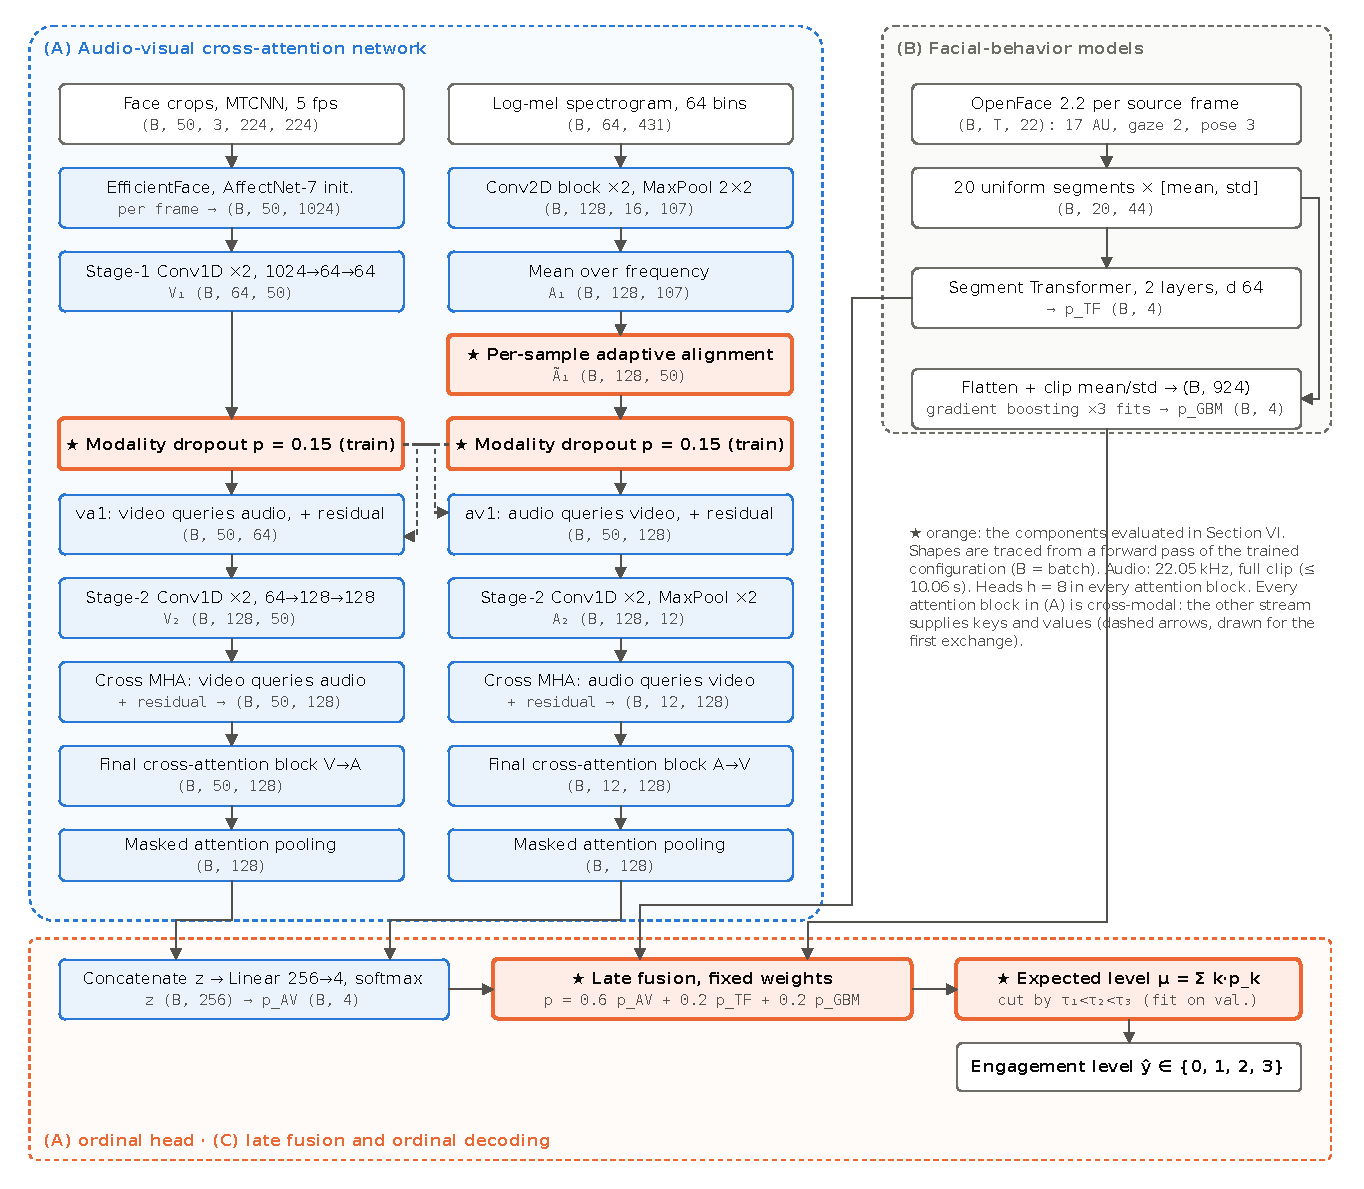
\includegraphics[width=\textwidth]{architecture}
\caption{Proposed \ournet{} architecture in detail. Tensor shapes are traced from a forward pass of the trained configuration ($B$ = batch). (A) Audio tokens are pooled onto the 50-step visual clock of the same clip before the first cross-attention exchange; after the second convolutional stage the audio stream has 12 tokens and the video stream 50; every attention block is cross-modal, and the final pair has no residual connection. (B) Two models on segment statistics of the per-frame OpenFace descriptor. (C) The three class-probability vectors are averaged with fixed weights, reduced to an expected level, and cut by thresholds fitted on the validation split. Orange blocks mark the components evaluated in Section~\ref{sec:results}}
\label{fig:arch}
\end{figure*}

\begin{algorithm}[t]
\caption{\ournet{} training and inference}\label{alg:ournet}
\begin{algorithmic}[1]
\Require face frames $\mathbf{I}$, log-mel spectrogram $\mathbf{X}_a$, OpenFace series $\mathbf{B}$, level $y$
\Ensure engagement level $\hat{y} \in \{0,1,2,3\}$
\For{each training iteration}
\State $\mathbf{V}_1 \gets \mathrm{Conv1D}(\mathrm{EfficientFace}(\mathbf{I}))$
\State $\tilde{\mathbf{A}}_1 \gets \mathrm{Align}(\mathrm{Conv2D}(\mathbf{X}_a), T_v)$
\State apply modality dropout ($p = 0.15$) to $\tilde{\mathbf{A}}_1$ and $\mathbf{V}_1$
\State $p_{\mathrm{AV}} \gets \mathrm{Network}(\tilde{\mathbf{A}}_1, \mathbf{V}_1)$ \Comment{three cross-modal exchanges}
\State compute $\mathcal{L}$ of (\ref{eq:loss}) and update the network
\EndFor
\State $\mathbf{S} \gets \mathrm{SegmentStatistics}(\mathbf{B}, 20)$
\State train the gradient-boosting model on $[\mathrm{flatten}(\mathbf{S}), \mathrm{clip\ statistics}]$ and the segment Transformer on $\mathbf{S}$
\State $p \gets 0.6\,p_{\mathrm{AV}} + 0.2\,p_{\mathrm{TF}} + 0.2\,p_{\mathrm{GBM}}$
\State fit $\tau_1 < \tau_2 < \tau_3$ on the validation split
\State $\hat{y} \gets \sum_{m} \mathbf{1}[\sum_k k\,p_k \ge \tau_m]$
\end{algorithmic}
\end{algorithm}

\subsection{Problem formulation}\label{sec:formulation}

Each sample is a clip of a student's webcam recording with face frames, an audio track and a per-frame facial-behavior descriptor. We write the label set as $\mathcal{Y} = \{0, 1, \ldots, K-1\}$ with $K = 4$, where larger values mean higher engagement. For a clip with label $y$, a model produces logits $z \in \mathbb{R}^{K}$ and class probabilities $p_k = \exp(z_k) / \sum_{j} \exp(z_j)$. The usual decision rule takes the largest probability,
\begin{equation}
\hat{y} = \arg\max_{k} \; p_k \label{eq:argmax}
\end{equation}
Here, $\hat{y}$ is the predicted level. This rule uses the value of each probability but not the position of each class on the scale. In order to use the position of each class, an ordered alternative first reduces the probability vector to the expected level using the following equation,
\begin{equation}
\mu = \sum_{k=0}^{K-1} k \, p_k \label{eq:mu}
\end{equation}
Here, $\mu$ is a continuous value in $[0, K-1]$. The expected level is then cut with increasing thresholds $\tau_1 < \tau_2 < \tau_3$, and the predicted level is calculated as,
\begin{equation}
\hat{y} = \sum_{m=1}^{K-1} \mathbf{1}\!\left[\mu \geq \tau_m\right] \label{eq:thresh}
\end{equation}
Here, $\mathbf{1}[\cdot]$ is the indicator function, so $\hat{y}$ is the number of thresholds that $\mu$ reaches. The thresholds are fitted on the validation split and are not learned during training. Threshold rules on a scalar engagement score are also used in CMOSE \citep{wu2024cmose}; here the scalar is the expected level of the class probabilities, so the rule can be applied to any classifier without retraining it. During training, the order can be used by adding to the cross-entropy loss $\mathcal{L}_{\mathrm{CE}}$ a penalty that grows with the distance between the predicted and the true level, using the following equation,
\begin{equation}
\mathcal{L} = \mathcal{L}_{\mathrm{CE}} + \lambda \sum_{k} p_k \left| c_k - c_y \right|, \qquad c_k = \frac{k}{K-1} \label{eq:loss}
\end{equation}
Here, $c_y$ is the position of the true level $y$, the class positions $c_k$ are normalized to $[0,1]$, and $\lambda$ sets the weight of the distance term; both terms are averaged over the mini-batch. In this work, we train the audio-visual network ($\lambda = 0.15$) and the segment-Transformer model with (\ref{eq:loss}), and we decode the fused class probabilities with (\ref{eq:mu}) and (\ref{eq:thresh}) instead of (\ref{eq:argmax}).

\subsection{Audio-visual cross-attention network}\label{sec:method_av}

We pick the intermediate cross-attention fusion of AVT-CA \citep{venkatraman2025avtca} for the audio-visual network because in this fusion each modality attends to the other at three stages of the network. The network predicts the engagement level of a clip from its face frames and its audio track, and it uses multi-head attention with $h = 8$ heads throughout.

\subsubsection{Audio encoder}\label{sec:audio}

The audio track of each clip is resampled to 22.05\,kHz and converted to a 64-bin log-mel spectrogram $\mathbf{X}_a \in \mathbb{R}^{64 \times 431}$ for a 10\,s clip. Two two-dimensional convolution blocks ($3 \times 3$ convolution, batch normalization, ReLU and $2 \times 2$ max pooling) with 64 and 128 channels operate over frequency and time, and the frequency axis is then averaged, which gives the first-stage audio tokens $\mathbf{A}_1 \in \mathbb{R}^{128 \times 107}$.

\subsubsection{Visual encoder}\label{sec:visual}

Each clip is sampled at 5 frames per second, which gives up to 50 face crops of $224 \times 224$ pixels detected with MTCNN \citep{zhang2016mtcnn}. We use an EfficientFace backbone \citep{zhao2021efficientface} to map each frame to a 1024-dimensional embedding. In order to start the visual encoder from a face-specific representation, the backbone is initialized from weights trained for seven-class facial expression recognition on AffectNet \citep{mollahosseini2019affectnet}. Two one-dimensional convolution blocks (convolution with kernel size 3, batch normalization and ReLU; 1024$\to$64$\to$64) over the stacked embeddings give the first-stage visual tokens $\mathbf{V}_1 \in \mathbb{R}^{64 \times T_v}$ with $T_v \le 50$.

\subsubsection{Per-sample temporal alignment}\label{sec:align}

Our intuition is to make each audio token describe the same span of the clip as one visual token before the two streams exchange information. Without this step, the 107 audio steps of a full clip describe it at about twice the temporal resolution of its 50 visual tokens, and each visual token attends over all of them. Therefore, we pool the valid audio steps of every sample onto the valid visual length of the same sample using the following equation,
\begin{equation}
\begin{split}
\tilde{\mathbf{A}}_1[:, j] &= \frac{1}{|S_j|}\sum_{t \in S_j} \mathbf{A}_1[:, t],\\
S_j &= \left\{ t : \left\lfloor \tfrac{(j-1)L_a}{T_v} \right\rfloor \le t < \left\lceil \tfrac{j L_a}{T_v} \right\rceil \right\}
\end{split}
\end{equation}
Here, $\tilde{\mathbf{A}}_1[:, j]$ is the $j$-th aligned audio token for $j = 1, \dots, T_v$, $L_a$ and $T_v$ are the numbers of valid audio steps and valid visual tokens of the sample, the valid audio steps are indexed $t = 0, \dots, L_a - 1$, and $S_j$ is the $j$-th window under the rule of adaptive average pooling: the windows are of nearly equal width, and adjacent windows may share one step. Padding steps are excluded before pooling and masked afterwards, so the alignment holds for clips of any length, and $\tilde{\mathbf{A}}_1 \in \mathbb{R}^{128 \times 50}$ for a full clip. Its effect on accuracy is not measured in this paper (Section~\ref{sec:limitations}).

\subsubsection{Cross-attention fusion}\label{sec:xattn}

Scaled dot-product attention \citep{vaswani2017attention} maps a query matrix $Q$, a key matrix $K$ and a value matrix $V$ to an output using the following equation,
\begin{equation}
\mathrm{Att}(Q,K,V) = \mathrm{softmax}\!\left(\frac{QK^{\top}}{\sqrt{d_h}}\right) V
\end{equation}
Here, $d_h = d_o / h$ is the size of one of the $h$ attention heads and $d_o$ is the output size. Multi-head attention applies this operation $h$ times with separate learned projections, $\mathrm{head}_i = \mathrm{Att}(X_q W_i^{Q}, X_k W_i^{K}, X_k W_i^{V})$, and concatenates the results, $\mathrm{MHA}(X_q, X_k) = [\mathrm{head}_1, \ldots, \mathrm{head}_h] W^{O}$, where $X_q$ supplies the queries and $X_k$ supplies the keys and the values. In cross-attention, the queries and the keys come from different streams, and the two directions with residual connections are calculated as,
\begin{align}
\tilde{X}_a &= X_a + \mathrm{MHA}(X_a, X_v) \label{eq:xattn_a}\\
\tilde{X}_v &= X_v + \mathrm{MHA}(X_v, X_a) \label{eq:xattn_v}
\end{align}
Here, $\tilde{X}_a$ and $\tilde{X}_v$ are the audio and video streams after the exchange; the attention matrix in (\ref{eq:xattn_a}) has shape $T_a \times T_v$, so the two lengths do not have to match. In the first and third exchanges, the attention is wrapped in a cross-attention block: layer normalization is applied to the query stream and to the key--value stream before the attention, the query, key and value projections have no bias, and the attended output is layer-normalized, passed through a two-layer feed-forward network (hidden width $2d_o$, GELU activation) and added back to itself. Each block projects to the width of its query stream, so $d_o = 128$ when the audio tokens are the queries and $d_o = 64$ when the first-stage visual tokens are the queries, and no dropout is used inside the blocks. The three exchanges are as follows.

\emph{First exchange.} The aligned audio tokens query the visual tokens and the visual tokens query the audio tokens, with $X_a = \tilde{\mathbf{A}}_1$ and $X_v = \mathbf{V}_1$ in (\ref{eq:xattn_a}) and (\ref{eq:xattn_v}); the block outputs are added to the streams as the equations state.

\emph{Second stage and second exchange.} Each stream then passes through a second convolutional stage. Two one-dimensional convolution blocks (128$\to$256$\to$128, each with batch normalization, ReLU and max pooling with window 2) bring the audio tokens to $\mathbf{A}_2 \in \mathbb{R}^{128 \times 12}$, and two convolution blocks without pooling (64$\to$128$\to$128) bring the visual tokens to $\mathbf{V}_2 \in \mathbb{R}^{128 \times 50}$. In the second exchange, a standard multi-head attention layer in each direction, with biased projections and without the normalization and feed-forward sub-layers of the blocks above, lets the 12 audio tokens attend to the 50 visual tokens and the reverse; the attended output passes through dropout of 0.1 and is added to the stream.

\emph{Third exchange and pooling.} A final pair of cross-attention blocks forms the third exchange, this time without a residual connection: the audio stream is replaced by the output of the block in which the audio tokens are the queries and the visual tokens supply the keys and values, and the visual stream is replaced by the output of the reverse block. Each stream therefore ends as a summary of the other stream, weighted by the attention of its own tokens. Each stream is reduced over time to a 128-dimensional vector by masked attention pooling, in which a linear layer scores each valid time step and the tokens are averaged under the softmax of these scores. The two vectors are concatenated into the audio-visual summary $\mathbf{z} \in \mathbb{R}^{256}$, and a linear layer maps $\mathbf{z}$ to the four class probabilities $p_{\mathrm{AV}}$.

\subsubsection{Modality dropout and training objective}\label{sec:dropout}

In order to prevent the network from relying on only one stream, during training we set the entire token sequence of each modality to zero with probability $p = 0.15$ per sample, independently for audio and video, at the point where the first exchange begins. As with the alignment, we did not ablate this step, but it makes the inference-time modality ablation of Section~\ref{sec:abl_modality} a condition that the network has seen in training. The network is trained with the objective of (\ref{eq:loss}), with label smoothing of 0.1 in $\mathcal{L}_{\mathrm{CE}}$ and $\lambda = 0.15$, so that probability mass placed three levels from the true level costs more than mass placed one level away.

\subsection{Facial-behavior models}\label{sec:method_beh}

The second block predicts the engagement level from explicit facial-behavior descriptors of the same clip. We pick OpenFace descriptors for this block because the best EngageNet baseline uses them \citep{singh2023engagenet} and because gradient boosting on action units has worked well in earlier engagement studies \citep{das2025optimizing,wang2026shap}.

\subsubsection{Segment statistics}\label{sec:segstats}

OpenFace 2.2 \citep{baltrusaitis2018openface} is run on the source video of each clip and gives, per frame, 17 action-unit intensities, two gaze angles and three head-pose rotations, a 22-channel series $\mathbf{B} \in \mathbb{R}^{T \times 22}$. Following the best EngageNet baseline \citep{singh2023engagenet}, the series is divided into $S = 20$ segments of equal length, and each segment is described by the mean and standard deviation of every channel, which gives a $20 \times 44$ token sequence $\mathbf{S}$.

\subsubsection{Gradient-boosting model}\label{sec:gbm}

The 20 tokens are flattened and extended with the mean and standard deviation of each channel over the whole clip, a 924-dimensional vector. A histogram gradient-boosting classifier \citep{pedregosa2011sklearn} with at most 15 leaves per tree and L2 regularization of 1.0 is trained on this vector. Three fits with learning rate and iteration count (0.05, 300), (0.03, 600) and (0.05, 300) and different random seeds are averaged to give $p_{\mathrm{GBM}}$.

\subsubsection{Segment-Transformer model}\label{sec:segtf}

A pre-norm Transformer encoder \citep{vaswani2017attention} with a class token and learned positional embeddings reads the 20 tokens of $\mathbf{S}$ and outputs $p_{\mathrm{TF}}$. It is trained with the objective of (\ref{eq:loss}) and label smoothing of 0.1, the AdamW optimizer with a warm-up cosine schedule, and random dropout of segment tokens. Its size (two layers, model width 64, feed-forward width 128) was selected from eight candidate configurations by mean validation accuracy over three seeds.

\subsection{Late fusion and ordinal decoding}\label{sec:method_fusion}

The third block combines the class-probability vectors of the three models by a weighted average, which is calculated as,
\begin{equation}
p = w_{\mathrm{AV}}\, p_{\mathrm{AV}} + w_{\mathrm{TF}}\, p_{\mathrm{TF}} + w_{\mathrm{GBM}}\, p_{\mathrm{GBM}} \label{eq:late}
\end{equation}
Here, $p_{\mathrm{AV}}$, $p_{\mathrm{TF}}$ and $p_{\mathrm{GBM}}$ are the class-probability vectors of the audio-visual network, the segment Transformer and the gradient-boosting model. The weights $(w_{\mathrm{AV}}, w_{\mathrm{TF}}, w_{\mathrm{GBM}})$ are fixed to $(0.6, 0.2, 0.2)$ for every seed. This is the setting that a grid search on the validation split selected for seven of the eight networks we fused with the two behavior models: the three seeds of the audio-visual network, three seeds of the behavior-branch network of Section~\ref{sec:abl_branch}, and two seeds of its variant with action-unit text. Fusing at the probability level keeps the three models independent of each other, and Section~\ref{sec:res_sota} shows that many clips misclassified by the network are classified correctly by a behavior model. The fused vector $p$ is reduced to the expected level of (\ref{eq:mu}) and cut by the three thresholds of (\ref{eq:thresh}), which are fitted on the validation split only and applied unchanged to the test split. The fit is a coordinate search: starting from $(0.5, 1.5, 2.5)$, each threshold in turn is moved over a window of $\pm 1.0$ in steps of 0.01 while the other two are held fixed and the order of the thresholds is kept, for three rounds, and the setting with the highest validation top-1 accuracy is retained, with ties broken by adjacent accuracy and then by mean absolute error. For the network alone we compare four decoders: argmax (\ref{eq:argmax}), argmax after a per-class logit bias fitted on validation (a grid from $-2$ to $2$ in steps of 0.1 for levels 1--3, with level 0 fixed at 0), expected-level thresholds fitted on a grid with step 0.05, and refined expected-level thresholds obtained by a local search with radius 0.15 and step 0.005.

\section{Experiments}\label{sec:exp}

\subsection{Dataset}\label{sec:dataset}

We evaluate \ournet{} on EngageNet \citep{singh2023engagenet}, the online-learning engagement dataset with the largest number of participants. In EngageNet, the participants, aged 18 to 37, used a web-based platform with their own computer and webcam at sites such as computer labs, dorm rooms and open spaces; the videos were recorded at 640$\times$480 pixels or higher, and some contain background noise. The recordings are divided into 11,311 ten-second clips (31\,h) of 127 participants. In all experiments, we use the official subject-independent split, which assigns 90, 11 and 26 participants to training, validation and test (7,983, 1,071 and 2,257 clips). Every source clip is at most 10.06\,s long (median 10.00\,s), so the full clip is used for both modalities. We exclude the 105 clips that the dataset labels as ``subject not present'' (104 training clips and 1 test clip), since they carry no engagement level. Table~\ref{tab:dataset} shows the number of clips of each engagement level in the three splits. The \emph{highly engaged} level accounts for 50.27\% of the test clips (1,134 of 2,256), so a constant majority-class predictor scores 50.27\% top-1 accuracy and 16.73 macro-F1; every result in this paper is read against this reference.

\begin{table*}[t]
\caption{EngageNet clips used in this work, by engagement level (levels 0--3: not engaged, barely engaged, engaged, highly engaged)}\label{tab:dataset}
\begin{tabular*}{\textwidth}{@{\extracolsep\fill}lrrrrrr}
\toprule
Split & Participants & Clips & Level 0 & Level 1 & Level 2 & Level 3\\
\midrule
Training & 90 & 7,879 & 1,446 & 1,035 & 1,658 & 3,740\\
Validation & 11 & 1,071 & 132 & 97 & 273 & 569\\
Test & 26 & 2,256 & 457 & 246 & 419 & 1,134\\
\midrule
Share of test (\%) & & & 20.3 & 10.9 & 18.6 & 50.3\\
\botrule
\end{tabular*}
\end{table*}

\subsection{Compared methods}\label{sec:baselines}

We compare \ournet{} with the six baselines released with EngageNet \citep{singh2023engagenet}, which are, to our knowledge, the only published results on the official test split (Section~\ref{sec:rw_engagenet}). Four of them, an LSTM, a CNN-LSTM, a temporal convolutional network (TCN) and a Transformer encoder, read the OpenFace gaze, head-pose and action-unit features of each clip summarized by their mean and standard deviation over time windows, 98 values per window; the Transformer reads 20 windows of equal duration, the tokenization that our segment statistics follow. The fifth baseline is the same Transformer on MARLIN video features, and the sixth fuses the two feature sets. We take the test accuracies of the six baselines from the EngageNet paper and do not retrain them, so the comparison uses the same split and the same labels, but the authors' own training. The majority-class predictor of Section~\ref{sec:dataset} is the second reference. The later EngageNet results in Table~\ref{tab:related} are on other splits and are not compared.

\subsection{Implementation details}\label{sec:impl}

We trained the audio-visual network, the gradient-boosting model and the segment Transformer separately; Table~\ref{tab:config} lists the configuration of each. All clips are processed identically across the three splits. We sampled the face frames at 5 frames per second, detected the faces with MTCNN \citep{zhang2016mtcnn}, and cropped and resized them to $224 \times 224$ pixels; a clip with more than 50 frames is subsampled uniformly to 50, and a clip with fewer is padded with masked frames. The audio track is resampled to 22.05\,kHz and converted to the 64-bin log-mel spectrogram of Section~\ref{sec:audio}. We collected the facial-behavior series with OpenFace 2.2 \citep{baltrusaitis2018openface}, which detects a face in 98.2\% of the frames. Before the reported fine-tuning, the network was trained on EngageNet in three stages starting from the AffectNet initialization of the visual backbone, with the audio and fusion modules initialized randomly: 30 epochs with the cross-entropy loss at a learning rate of $10^{-2}$ and batch size 2, then 25 epochs with the ordinal objective at $10^{-4}$ and batch size 2, and then 8 epochs with the ordinal objective at $5 \times 10^{-5}$ and batch size 8, each stage starting from the weights of the previous one. These stages read every face frame of a clip, and the class-balanced sampler was used in the reported fine-tuning only.
All reported networks are fine-tuned from the resulting checkpoint with three random seeds; each fine-tuning run took about 32 minutes on a single NVIDIA RTX 3090 GPU with 24\,GB of memory. The two behavior models were trained on the training split only: the segment Transformer on the same GPU and the gradient-boosting model on the CPU. The networks were implemented in PyTorch 2.5 and the gradient-boosting model in scikit-learn \citep{pedregosa2011sklearn}. The test split is used only for the final evaluation: the kept checkpoint of each run, the size of the segment Transformer, the fusion weights and the decoding thresholds are all chosen on the validation split, and each reported test result is computed once. Generative AI was used in preparing this study as described in the AI declaration in the Statements and Declarations; it did not produce data, and every reported number was computed by the authors' code from the trained models.

\begin{table*}[t]
\caption{Training configuration of the three models}\label{tab:config}
\begin{tabular*}{\textwidth}{@{\extracolsep\fill}llll}
\toprule
Setting & Audio-visual network & Segment Transformer & Gradient boosting\\
\midrule
Input & 50 face frames + log-mel & 20 tokens (44-d) & 924-d vector\\
Optimizer & SGD, momentum 0.9 & AdamW & --\\
Learning rate & $5 \times 10^{-5}$, constant & $10^{-3}$, warm-up cosine & 0.05 / 0.03 / 0.05\\
Weight decay / L2 & $10^{-3}$ & 0.05 & 1.0\\
Batch size & 8 & 64 & --\\
Epochs / iterations & 6 (fine-tuning) & 60 & 300 / 600 / 300\\
Loss & CE + ordinal & CE + ordinal & log loss\\
Ordinal weight $\lambda$ & 0.15 & 0.15 & --\\
Label smoothing & 0.1 & 0.1 & --\\
Sampling & inverse-sqrt class frequency & uniform & uniform\\
Dropout & modality 0.15 & 0.3, token 0.1 & --\\
Tree size & -- & -- & $\le$ 15 leaves\\
Seeds & 3 & 3 & 3 fits averaged\\
\botrule
\end{tabular*}
\end{table*}

\subsection{Evaluation metrics}\label{sec:metrics}

We use four metrics. Let $N$ be the number of test clips, with true levels $y_i$ and predictions $\hat{y}_i$, and let $\mathbf{1}[\cdot]$ denote the indicator function. Top-1 accuracy is the fraction of test clips whose predicted level matches the annotated level, calculated as
\begin{equation}
\mathrm{Top\text{-}1} = \frac{1}{N} \sum_{i=1}^{N} \mathbf{1}[\hat{y}_i = y_i].
\label{eq:top1}
\end{equation}
It is the metric reported by every EngageNet study reviewed in Section~\ref{sec:related}, and it scores a prediction one level from the truth in the same way as a prediction three levels from the truth. Adjacent accuracy is the fraction of clips predicted within one level of the truth,
\begin{equation}
\mathrm{Adj} = \frac{1}{N} \sum_{i=1}^{N} \mathbf{1}[|\hat{y}_i - y_i| \leq 1];
\label{eq:adj}
\end{equation}
none of the EngageNet studies we reviewed reports it. The mean absolute error is the average distance in levels between the prediction and the truth,
\begin{equation}
\mathrm{MAE} = \frac{1}{N} \sum_{i=1}^{N} |\hat{y}_i - y_i|,
\label{eq:mae}
\end{equation}
so a value of 0.40 means that a prediction is on average 0.40 levels from the truth. Macro-F1 is the unweighted mean of the per-level F1 scores,
\begin{equation}
\mathrm{F1}_k = \frac{2\,P_k R_k}{P_k + R_k}, \qquad \mathrm{Macro\text{-}F1} = \frac{1}{K} \sum_{k=0}^{K-1} \mathrm{F1}_k,
\label{eq:f1}
\end{equation}
where $P_k$ and $R_k$ are the precision and recall of level $k$ and $K = 4$ is the number of levels. Because it weights the four levels equally, it cannot be raised by predicting the majority level. High values are preferred for top-1, adjacent accuracy and macro-F1, and a low value for MAE. Unless stated otherwise, a result is the mean over three seeds on the 2,256 test clips, the network alone is decoded with its refined expected-level thresholds, and $\pm$ values are standard deviations over seeds.

\section{Results and discussion}\label{sec:results}

\subsection{Comparison with published EngageNet results}\label{sec:res_sota}

\begin{figure*}[t]
\centering
% Fig. -- test top-1 on EngageNet. Error bars: sd over 3 seeds (ours). Grey = published (Singh et al., ICMI 2023).
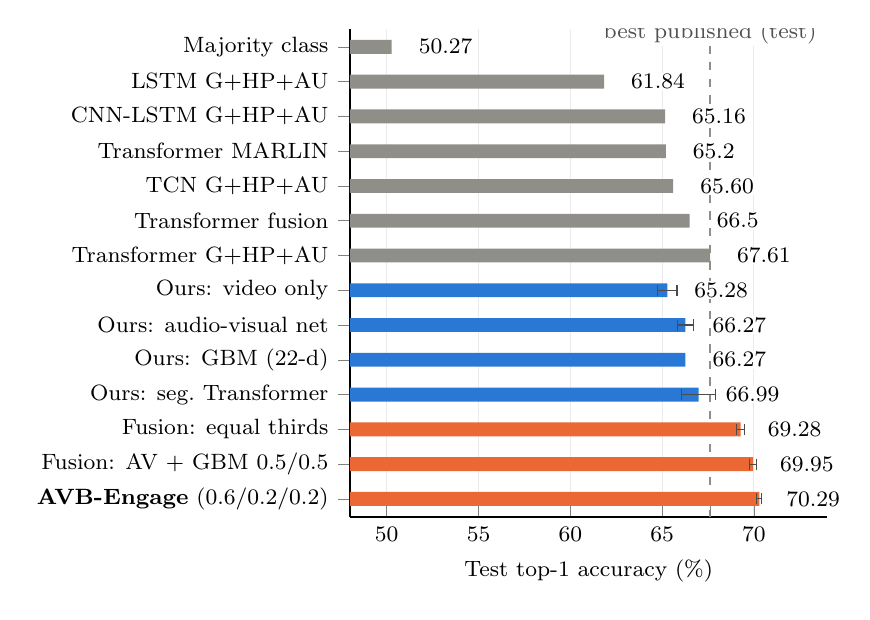
\begin{tikzpicture}
\begin{axis}[
  xbar, bar shift=0pt, scale only axis, width=0.5\textwidth, height=6.2cm, bar width=5pt,
  xmin=48, xmax=74, xlabel={Test top-1 accuracy (\%)}, xlabel style={font=\footnotesize},
  ytick={maj,lstm,cnnlstm,marlin,tcn,tffus,tfbest,vonly,av,gbm,tf,eq3,av2,w3}, yticklabel style={font=\footnotesize, align=right}, xticklabel style={font=\footnotesize},
  symbolic y coords={maj,lstm,cnnlstm,marlin,tcn,tffus,tfbest,vonly,av,gbm,tf,eq3,av2,w3},
  yticklabels={Majority class,LSTM {\footnotesize G+HP+AU},CNN-LSTM {\footnotesize G+HP+AU},Transformer {\footnotesize MARLIN},TCN {\footnotesize G+HP+AU},Transformer fusion,Transformer {\footnotesize G+HP+AU},Ours: video only,Ours: audio-visual net,Ours: GBM (22-d),Ours: seg.\ Transformer,Fusion: equal thirds,Fusion: AV + GBM 0.5/0.5,\textbf{AVB-Engage} (0.6/0.2/0.2)},
  y dir=reverse, enlarge y limits=0.04,
  axis x line*=bottom, axis y line*=left, xmajorgrids, grid style={draw=black!8},
  nodes near coords, nodes near coords style={font=\footnotesize, text=black, anchor=west, xshift=9pt, fill=white, inner sep=0.6pt},
  point meta=explicit symbolic,
  error bars/x dir=both, error bars/x explicit, error bars/error bar style={black!70},
  extra x ticks={67.61}, extra x tick labels={}, extra x tick style={grid=major, grid style={dashed, published, thick}},
]
\addplot[fill=published, draw=none] coordinates {
  (50.27,maj)[50.27] (61.84,lstm)[61.84] (65.16,cnnlstm)[65.16] (65.20,marlin)[65.2]
  (65.60,tcn)[65.60] (66.50,tffus)[66.5] (67.61,tfbest)[67.61]};
\addplot[fill=ours, draw=none] coordinates {
  (65.28,vonly) +- (0.53,0) [65.28] (66.27,av) +- (0.45,0) [66.27]
  (66.27,gbm)[66.27] (66.99,tf) +- (0.93,0) [66.99]};
\addplot[fill=fused, draw=none] coordinates {
  (69.28,eq3) +- (0.23,0) [69.28] (69.95,av2) +- (0.20,0) [69.95] (70.29,w3) +- (0.14,0) [70.29]};
\node[font=\footnotesize, text=inkmuted, anchor=south, fill=white, inner sep=1pt] at (axis cs:67.61,maj) {best published (test)};
\end{axis}
\end{tikzpicture}

\caption{Test top-1 accuracy on EngageNet compared with the published test-split baselines. Grey: baselines as reported by \citet{singh2023engagenet}, all video-only (we did not re-run them); G, HP and AU denote gaze, head-pose and action-unit features, and the Transformer fusion uses G+HP+AU and MARLIN features. For the LSTM we show the G+HP+AU result used in the comparison of \citet{singh2023engagenet}; its best test result there is 62.46\% with head pose only. The dashed line marks the best baseline (67.61\%). Blue: our single models. Orange: probability-level fusions of our models, the last being \ournet. Error bars are standard deviations over three seeds; the gradient-boosting model is a single averaged model}
\label{fig:results}
\end{figure*}

We compared \ournet{} and its components with the six baselines released with EngageNet and present the results in Fig.~\ref{fig:results}. As noted in Section~\ref{sec:rw_engagenet}, the later results in Table~\ref{tab:related} are on other splits and are not comparable. \ournet{} achieves the highest top-1 accuracy, 70.29 $\pm$ 0.14\%, against 67.61\% for the best baseline. The audio-visual network alone reaches 66.27 $\pm$ 0.45\%, above four of the six baselines but below the best one. The gradient-boosting model and the segment Transformer, which read only 22 of the 98 OpenFace features used by the best baseline, reach the same range as the network (66.27\% and 66.99\%). The fusion gain comes from errors that the models do not share: the network and the gradient-boosting model are each wrong on about 34\% of the test clips, but both are wrong on only about 22\%.

Two points qualify this comparison. First, it is not like-for-like: \ournet{} averages three models and fits its decoding thresholds on the validation split, whereas each baseline is a single model decoded from its softmax output. Second, the best baseline is not a strong bound for its own features. A gradient-boosting model on the same 98 OpenFace features reaches 68.13\% with argmax decoding and 68.88\% with expected-level thresholds (Section~\ref{sec:abl_fusion}), so part of the margin of \ournet{} comes from the learner and the decoding rule rather than from the audio-visual network.

\subsection{Per-seed and per-level results}\label{sec:res_seed}

Table~\ref{tab:seeds} reports every model per seed with the four metrics. \ournet{} has the highest top-1 accuracy and macro-F1, the lowest mean absolute error and the smallest standard deviation over seeds of all trained models. The audio-visual network has a slightly higher adjacent accuracy than \ournet. For every trained model the adjacent accuracy is more than 20 points above the top-1 accuracy, so most errors are one-level errors.

\begin{table*}[t]
\caption{Test results per seed (top-1, \%) and mean over three seeds. The network rows with one input at inference are the ablation of Section~\ref{sec:abl_modality}; the gradient-boosting model is one averaged model}\label{tab:seeds}
\begin{tabular*}{\textwidth}{@{\extracolsep\fill}lccccccc}
\toprule
Model & Seed 1 & Seed 2 & Seed 3 & Top-1 & Adj. & MAE & Macro-F1\\
\midrule
Majority-class predictor & 50.27 & 50.27 & 50.27 & 50.27 & 68.84 & 1.012 & 16.73\\
Network, audio only & 46.59 & 50.27 & 50.27 & 49.04 $\pm$ 2.12 & 69.27 & 1.004 & 17.35\\
Network, video only & 65.60 & 65.56 & 64.67 & 65.28 $\pm$ 0.53 & 90.77 & 0.459 & 51.29\\
Audio-visual network & 65.78 & 66.36 & 66.67 & 66.27 $\pm$ 0.45 & \textbf{91.55} & 0.440 & 52.31\\
Gradient boosting & 66.27 & 66.27 & 66.27 & 66.27 & 89.01 & 0.476 & 50.04\\
Segment Transformer & 67.02 & 67.91 & 66.05 & 66.99 $\pm$ 0.93 & 87.90 & 0.487 & 49.45\\
\textbf{\ournet} & 70.17 & 70.26 & 70.43 & \textbf{70.29 $\pm$ 0.14} & 91.06 & \textbf{0.401} & \textbf{53.95}\\
\botrule
\end{tabular*}
\end{table*}

Table~\ref{tab:levels} reports precision, recall and F1 per level. The two extreme levels are recognized well by every model, and the two middle levels are not. The three models fail on the middle levels in different ways: the gradient-boosting model almost never predicts \emph{barely engaged} (recall 1.6\%) but has the highest recall on \emph{engaged} (59.4\%), whereas the network has the highest recall on \emph{barely engaged} (17.8\%). Fusion raises the F1 of \emph{engaged} from 28.8 to 39.8 and of \emph{highly engaged} from 80.3 to 85.1, and lowers the F1 of \emph{barely engaged} from 22.3 to 15.4.

\begin{table*}[t]
\caption{Precision (P), recall (R) and F1 per engagement level on the test split (\%, mean of three seeds)}\label{tab:levels}
\setlength{\tabcolsep}{3pt}
\begin{tabular*}{\textwidth}{@{\extracolsep\fill}lcccccccccccc}
\toprule
& \multicolumn{3}{c}{Not engaged} & \multicolumn{3}{c}{Barely engaged} & \multicolumn{3}{c}{Engaged} & \multicolumn{3}{c}{Highly engaged}\\
\cmidrule{2-4}\cmidrule{5-7}\cmidrule{8-10}\cmidrule{11-13}
Model & P & R & F1 & P & R & F1 & P & R & F1 & P & R & F1\\
\midrule
Audio-visual network & 78.9 & 76.8 & \textbf{77.8} & 30.6 & 17.8 & \textbf{22.3} & 32.5 & 25.9 & 28.8 & 74.3 & 87.4 & 80.3\\
Gradient boosting & 71.3 & 67.4 & 69.3 & 44.4 & 1.6 & 3.1 & 37.5 & 59.4 & \textbf{46.0} & 81.1 & 82.4 & 81.8\\
Segment Transformer & 63.2 & 68.9 & 65.9 & 23.0 & 5.1 & 8.4 & 40.6 & 39.2 & 39.7 & 78.6 & 89.9 & 83.8\\
\ournet & 78.5 & 73.0 & 75.5 & 32.4 & 10.6 & 15.4 & 42.1 & 37.7 & 39.8 & 77.6 & 94.2 & \textbf{85.1}\\
\botrule
\end{tabular*}
\end{table*}

\subsection{Effect of the decoding rule}\label{sec:res_decoder}

Table~\ref{tab:decoder} isolates the decoding rule of Section~\ref{sec:formulation} on the audio-visual network. Replacing argmax with expected-level thresholds adds 2.00 points of top-1 accuracy for the network and 1.80 points for its video-only condition, with no change to the weights and no test data used in the fit. This gain is larger than the effect of any single training change in Section~\ref{sec:abl_sweep}, and larger than the gap between most of the published baselines, which decode a softmax output with argmax.

\begin{table*}[t]
\caption{Effect of the decoding rule on the same trained weights (test top-1, \%, three seeds)}\label{tab:decoder}
\begin{tabular*}{\textwidth}{@{\extracolsep\fill}lcc}
\toprule
Decoder & Audio + video & Video only\\
\midrule
Argmax & 64.27 $\pm$ 0.22 & 63.48 $\pm$ 0.35\\
Fitted logit bias & 65.06 $\pm$ 0.37 & 63.83 $\pm$ 0.45\\
Expected-level thresholds & \textbf{66.34 $\pm$ 0.50} & 65.26 $\pm$ 0.40\\
Refined expected-level thresholds & 66.27 $\pm$ 0.45 & \textbf{65.28 $\pm$ 0.53}\\
\midrule
Refined thresholds $-$ argmax & +2.00 & +1.80\\
\botrule
\end{tabular*}
\end{table*}

\subsection{Ablation studies}\label{sec:ablation}

We performed five separate ablation studies on the EngageNet test split. Three seeds of one configuration give a standard deviation of 0.45 points of top-1 accuracy and about 1.1 points of macro-F1, and the binomial 95\% confidence interval on 2,256 test clips is about $\pm$1.95 points. We therefore treat a difference in three-seed means below about one point as within noise, and use the consistency of sign across matched models for smaller effects.

\subsubsection{Contribution of each modality}\label{sec:abl_modality}

Instead of training separate unimodal models, which would change the optimization run as well as the input, we kept the trained weights unchanged and set the token sequence of one modality to zero at inference, the same operation as modality dropout. We applied this to the nine fine-tuned networks of this work: three seeds each of the audio-visual network and of the two behavior-branch variants of Section~\ref{sec:abl_branch}. Audio alone scores at or below the majority-class predictor in all nine networks (Table~\ref{tab:modality}), so audio by itself does not predict engagement on this dataset. Adding audio to video raises top-1 accuracy in seven of the nine networks, leaves it unchanged in one and lowers it by 0.13 points in one, by 0.74 points on average. Only one difference (1.99 points) reaches the 95\% interval of a single test evaluation, so the evidence is the consistent sign rather than any single network. The nine networks share one warm start and are therefore not independent samples. An earlier sweep of thirteen networks fine-tuned from the same warm start gives the same picture, with the audio-visual input higher in twelve of the thirteen (0.67 points on average), but it is not an independent replication either. Macro-F1 is higher with audio in six of the nine networks.

\begin{table*}[t]
\caption{Inference-time modality ablation on the same trained weights (nine networks, test top-1, \%)}\label{tab:modality}
\begin{tabular*}{\textwidth}{@{\extracolsep\fill}lcc}
\toprule
Input at inference & Mean top-1 & Audio + video higher in\\
\midrule
Audio + video & \textbf{66.16} & --\\
Video only & 65.41 & 7 of 9 (1 tie)\\
Audio only & 48.60 & 9 of 9\\
\botrule
\end{tabular*}
\end{table*}

\subsubsection{Behavior branch inside the network}\label{sec:abl_branch}

We tested whether the facial-behavior descriptors can be learned inside the network instead of in separate models. We attached a behavior branch to the same warm start as the audio-visual network. A one-dimensional convolution (22$\to$128) and a bidirectional GRU encode the OpenFace series, resampled to the 50-step visual clock. The audio-visual summary $\mathbf{z}$ is projected to a query that attends over these behavior tokens, and the clip mean of the descriptor passes through a linear layer to a 64-dimensional vector. The classifier reads the concatenation of $\mathbf{z}$, the attended behavior vector and this clip-level vector. The new classifier columns were initialized to zero, so that at the start of fine-tuning the model is exactly the audio-visual network (maximum logit difference 0.0), and the branch was fine-tuned with the same schedule and seeds. We also tested a second variant that adds a text rendering of the same action-unit series as a further input. Neither variant changes any metric by more than a fraction of the seed standard deviation (Table~\ref{tab:branch}). The same descriptors raise accuracy when they are used through the separate models of block B: with a behavior-branch network in place of the audio-visual network as the neural member of the fusion, the fused accuracy is 69.9--70.4\% over three seeds. The descriptors are therefore informative, and the per-frame recurrent branch does not extract what the segment statistics provide.

\begin{table*}[t]
\caption{Behavior branch inside the network (test, three seeds)}\label{tab:branch}
\begin{tabular*}{\textwidth}{@{\extracolsep\fill}lcccc}
\toprule
Network & Top-1 & Adj. & MAE & Macro-F1\\
\midrule
Audio-visual & \textbf{66.27 $\pm$ 0.45} & 91.55 & 0.440 & \textbf{52.31}\\
+ behavior branch & 66.08 $\pm$ 0.59 & 91.62 & 0.441 & 52.16\\
+ branch + AU text & 66.12 $\pm$ 0.59 & \textbf{91.67} & \textbf{0.439} & 52.26\\
\botrule
\end{tabular*}
\end{table*}

\subsubsection{Fusion weights}\label{sec:abl_fusion}

We evaluated the fusion of block C under different weight rules, keeping all three models unchanged (Table~\ref{tab:fusion}). Every rule and every seed gives between 67.4\% and 70.5\%; the lowest values occur when validation selected a weight of 0.8 or more for the network on one seed. Equal weights, which involve no selection, give 69.28 $\pm$ 0.23\%. Fusing the network with the segment Transformer alone is unstable across seeds (68.69 $\pm$ 2.08\% with validation-selected weights), because the validation accuracy of the Transformer does not follow its test accuracy closely; adding the gradient-boosting model reduces the standard deviation to 0.14 points. Fig.~\ref{fig:sensitivity} shows that accuracy changes little for network weights between 0.5 and 0.7 and drops once the network dominates the average. Finally, we replaced the 22-dimensional descriptor with the full 98-dimensional OpenFace descriptor of the best baseline. The gradient-boosting model alone then reaches 68.88\% (68.13\% with argmax decoding), above the published Transformer on the same features, but the three-way fusion does not improve (69.15 $\pm$ 0.83\% over the eight networks of Section~\ref{sec:method_fusion}, with validation-selected weights).

\begin{table*}[t]
\caption{Late fusion under different weight rules (test top-1, \%, three seeds)}\label{tab:fusion}
\begin{tabular*}{\textwidth}{@{\extracolsep\fill}llc}
\toprule
Members & Weight rule & Top-1\\
\midrule
Network + GBM & fixed 0.5 / 0.5 & 69.95 $\pm$ 0.20\\
Network + GBM & fixed 0.7 / 0.3 & 70.04 $\pm$ 0.20\\
Network + GBM & selected on validation & 69.86 $\pm$ 0.50\\
Network + TF + GBM & fixed equal thirds & 69.28 $\pm$ 0.23\\
Network + TF + GBM & \textbf{fixed 0.6 / 0.2 / 0.2} & \textbf{70.29 $\pm$ 0.14}\\
Network + TF + GBM & selected on validation & 69.43--70.29\\
\botrule
\end{tabular*}
\end{table*}

\begin{figure*}[t]
\centering
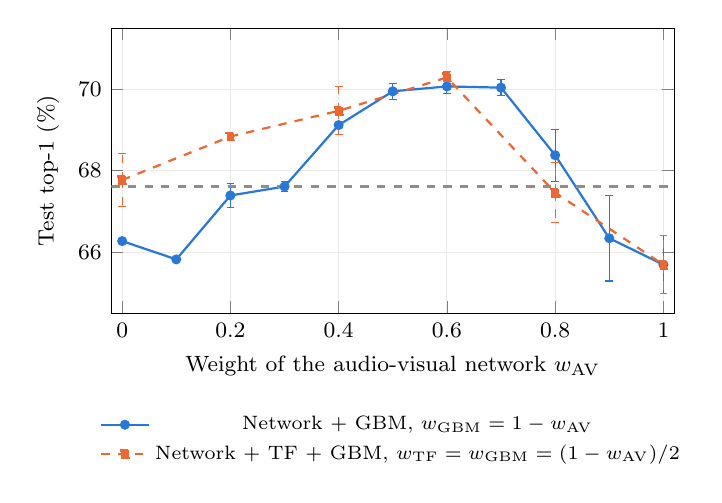
\begin{tikzpicture}
\begin{axis}[width=0.72\textwidth, height=5.2cm, xmin=-0.02, xmax=1.02, ymin=64.5, ymax=71.5,
  xlabel={Weight of the audio-visual network $w_{\mathrm{AV}}$}, ylabel={Test top-1 (\%)},
  label style={font=\footnotesize}, tick label style={font=\footnotesize}, legend style={font=\scriptsize, at={(0.5,-0.32)}, anchor=north, draw=none, legend columns=1},
  grid=major, grid style={draw=black!8}, error bars/y dir=both, error bars/y explicit]
\addplot[color=ours, mark=*, mark size=1.4pt, thick] coordinates {
 (0.0,66.27) +- (0,0) (0.1,65.82) +- (0,0.04) (0.2,67.39) +- (0,0.30) (0.3,67.61) +- (0,0.13) (0.4,69.12) +- (0,0.05)
 (0.5,69.95) +- (0,0.20) (0.6,70.07) +- (0,0.18) (0.7,70.04) +- (0,0.20) (0.8,68.38) +- (0,0.64) (0.9,66.34) +- (0,1.05) (1.0,65.69) +- (0,0.71)};
\addlegendentry{Network + GBM, $w_{\mathrm{GBM}} = 1 - w_{\mathrm{AV}}$}
\addplot[color=fused, mark=square*, mark size=1.4pt, thick, dashed] coordinates {
 (0.0,67.77) +- (0,0.66) (0.2,68.84) +- (0,0.08) (0.4,69.47) +- (0,0.59) (0.6,70.29) +- (0,0.14) (0.8,67.46) +- (0,0.73) (1.0,65.69) +- (0,0.71)};
\addlegendentry{Network + TF + GBM, $w_{\mathrm{TF}} = w_{\mathrm{GBM}} = (1 - w_{\mathrm{AV}})/2$}
\draw[dashed, published, thick] (axis cs:-0.02,67.61) -- (axis cs:1.02,67.61);
\end{axis}
\end{tikzpicture}
\caption{Sensitivity of the fused test top-1 accuracy to the fusion weights (mean $\pm$ standard deviation over three seeds; thresholds fitted on validation for every weight). The dashed grey line is the best published test result (67.61\%). At $w_{\mathrm{AV}} = 1$ the three network seeds are decoded with the fusion threshold search, which gives a mean of 65.69\% instead of the 66.27\% of their own refined thresholds}
\label{fig:sensitivity}
\end{figure*}

\subsubsection{Number of segments}\label{sec:abl_segments}

The segment statistics follow the 20-segment tokenization of the best EngageNet baseline. To test this choice, we re-ran the gradient-boosting model with the same recipe for $S \in \{1, 5, 10, 20, 40\}$ segments, keeping the segment Transformer at $S = 20$ (Table~\ref{tab:segments}). The number of segments changes the top-1 accuracy of the gradient-boosting model by about one point at most (0.80 points with argmax and 1.02 points with thresholds), and even $S = 1$, which keeps only the clip-level mean and standard deviation, reaches 67.29\% with threshold decoding. More segments raise its macro-F1 from 47.94 ($S = 1$) to 50.57 ($S = 40$). Every fused setting stays between 68.8\% and 70.6\%, so the result of \ournet{} does not depend on the choice of $S = 20$. We fixed $S = 20$ before this test to match the baseline and report it, rather than $S = 1$, which scores slightly higher on test, so that no design choice is made on the test split.

\begin{table*}[t]
\caption{Effect of the number of segments $S$ on the gradient-boosting model (test, \%). Fusions use the three network seeds (mean $\pm$ standard deviation) and fixed weights}\label{tab:segments}
\begin{tabular*}{\textwidth}{@{\extracolsep\fill}lcccccc}
\toprule
& & \multicolumn{3}{c}{Gradient boosting alone} & \multicolumn{2}{c}{Fused with the network}\\
\cmidrule{3-5}\cmidrule{6-7}
$S$ & Dims & Argmax & Thresholds & Macro-F1 & + GBM (0.5/0.5) & 3-way (0.6/0.2/0.2)\\
\midrule
1 & 88 & 66.89 & \textbf{67.29} & 47.94 & \textbf{69.96 $\pm$ 0.14} & \textbf{70.64 $\pm$ 0.24}\\
5 & 264 & 66.22 & 66.84 & 48.43 & 68.82 $\pm$ 1.26 & 70.54 $\pm$ 0.09\\
10 & 484 & 66.84 & 67.20 & 49.76 & 69.95 $\pm$ 0.35 & 70.24 $\pm$ 0.05\\
20 (reported) & 924 & 66.53 & 66.27 & 50.04 & 69.95 $\pm$ 0.20 & 70.29 $\pm$ 0.14\\
40 & 1804 & \textbf{67.02} & 66.71 & \textbf{50.57} & 69.86 $\pm$ 0.23 & 70.21 $\pm$ 0.12\\
\botrule
\end{tabular*}
\end{table*}

\subsubsection{Training variables of the network}\label{sec:abl_sweep}

We tested the training variables of the audio-visual network (Table~\ref{tab:sweep}). Fourteen fine-tuning runs were started from the same checkpoint: a control, three seeds of the class-balanced sampler, nine runs that each change one variable, and one run that adds synchronized random temporal cropping and lowers the video frame cap to 40. The nine single changes are the loss type, the ordinal penalty weight (two values), label smoothing, an exponential moving average of the weights, the learning-rate schedule, SpecAugment \citep{park2019specaugment} on the spectrogram, the video frame cap, and a class-weighted loss. The standard deviation across the fourteen runs (0.52 points) is close to the standard deviation across three seeds of one configuration (0.45 points). No change raises accuracy by more than the seed spread. Two single runs fall more than one point below the control: the class-weighted loss (64.72\%) and the frame cap of 40 with random cropping (64.89\%). Averaging the logits of all fourteen networks gives 65.69\%, below the best single network, which is consistent with networks fine-tuned from one checkpoint making similar errors. For a single network on this dataset, the training variables we tested do not raise top-1 accuracy beyond the seed noise; the gains in this paper come from the decoding rule and from combining different models.

\begin{table*}[t]
\caption{Single-variable fine-tuning sweep from one checkpoint (test, refined thresholds)}\label{tab:sweep}
\begin{tabular*}{\textwidth}{@{\extracolsep\fill}lcccc}
\toprule
Variable under test & Top-1 & Adj. & MAE & Macro-F1\\
\midrule
Control & 66.09 & 91.40 & 0.444 & 52.25\\
Balanced sampler, seed 1 & 65.78 & \textbf{92.24} & \textbf{0.436} & \textbf{53.41}\\
Balanced sampler, seed 2 & 66.36 & 91.09 & 0.444 & 51.13\\
Balanced sampler, seed 3 & \textbf{66.67} & 91.31 & 0.440 & 52.37\\
Loss = cross-entropy & 65.91 & 91.36 & 0.446 & 50.92\\
Ordinal weight 0.35 & 65.38 & 91.27 & 0.452 & 50.68\\
Ordinal weight 0.60 & 65.87 & 91.36 & 0.446 & 50.94\\
No label smoothing & 65.91 & 91.44 & 0.445 & 51.01\\
EMA 0.999 & 65.96 & 91.22 & 0.446 & 50.93\\
LR $10^{-4}$, warm-up cosine & 65.69 & 91.36 & 0.448 & 50.72\\
SpecAugment \citep{park2019specaugment} & 65.34 & 91.22 & 0.453 & 50.59\\
Frame cap 50 & 65.82 & 91.40 & 0.446 & 50.76\\
Frame cap 40 + random crop & 64.89 & 91.53 & 0.450 & 50.42\\
Class-weighted loss & 64.72 & 91.71 & 0.452 & 50.41\\
\midrule
Average of all 14 & 65.69 & -- & -- & --\\
\botrule
\end{tabular*}
\end{table*}

\subsection{Computational cost}\label{sec:res_cost}

Table~\ref{tab:cost} reports the size and inference cost of each component, measured on real test clips with batch size 1. The audio-visual network has 2.38\,M parameters, of which 1.26\,M are in the EfficientFace frame encoder, and needs 16.0\,GFLOPs per 10\,s clip, almost all of it in the frame encoder; the three cross-modal exchanges account for about 0.04\,GFLOPs. It processes a clip in 21.5\,ms on one RTX 3090 GPU and in 271\,ms on eight CPU threads. The two behavior models are small: the segment Transformer has 71,620 parameters, and the gradient-boosting model consists of 4,800 trees. The most expensive step of \ournet{} is not a model but the OpenFace extraction that feeds block B, which needed a median of 11.3\,s per clip on one CPU thread over 30 sampled test clips, about the duration of the clip itself. Real-time use therefore needs OpenFace to run on several threads or to be replaced by a faster facial-behavior extractor.

\begin{table*}[t]
\caption{Size and inference cost per 10\,s clip (batch size 1). GPU: NVIDIA RTX 3090; CPU timings use eight threads except OpenFace, which runs on one thread (median over 30 test clips). FLOPs count one multiply-add as two operations}\label{tab:cost}
\begin{tabular*}{\textwidth}{@{\extracolsep\fill}lcccc}
\toprule
Component & Parameters & FLOPs per clip & GPU time & CPU time\\
\midrule
Audio-visual network (total) & 2.38\,M & 16.0\,G & 21.5 $\pm$ 5.1\,ms & 271\,ms\\
\quad EfficientFace frame encoder & 1.26\,M & -- & -- & --\\
\quad Audio encoder & 0.27\,M & -- & -- & --\\
\quad Cross-attention blocks & 0.55\,M & 0.04\,G & -- & --\\
Segment Transformer & 71.6\,k & 0.11\,M & -- & 0.7\,ms\\
Gradient boosting (3 fits) & 4,800 trees & -- & -- & 38.6\,ms\\
OpenFace 2.2 extraction & -- & -- & -- & 11.3\,s\\
\botrule
\end{tabular*}
\end{table*}

\subsection{Error analysis}\label{sec:res_errors}

Both models fail mainly on the two middle levels. Fig.~\ref{fig:confusion} presents the row-normalized test confusion matrices of the audio-visual network and of \ournet, pooled over the three seeds. The network recognizes the two extreme levels in 77\% and 87\% of cases, but \emph{barely engaged} and \emph{engaged} in only 18\% and 26\%. Three quarters of its errors (74.9\%) are off by exactly one level, and two thirds (67.4\%) are on clips of the two middle levels, although these levels make up 29.5\% of the test set. \ournet{} shifts recall toward the upper half of the scale: it raises recall on \emph{highly engaged} from 87\% to 94\% and on \emph{engaged} from 26\% to 38\%, and lowers it on \emph{not engaged} from 77\% to 73\% and on \emph{barely engaged} from 18\% to 11\%. As a result, an even larger share of its errors (71.8\%) is on the two middle levels.

\begin{figure}[t]
\centering
% Fig. -- row-normalised test confusion matrices (%), pooled over the three seeds (3 x 2,256 clips).
% Values: results/paper_springer/analysis.json (rounded once from the counts) (scripts/paper/springer_analysis.py). Network decoded with its
% refined expected-level thresholds; fusion with thresholds fitted on validation (fixed 0.6/0.2/0.2).
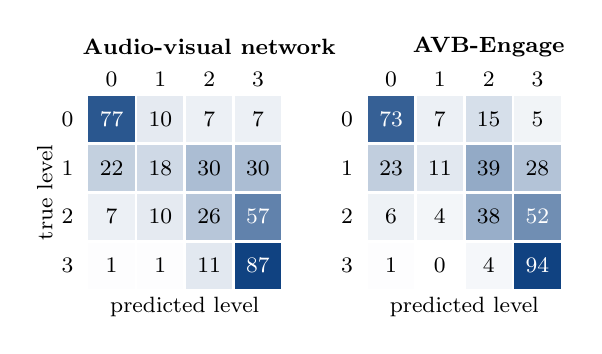
\begin{tikzpicture}[font=\footnotesize, cell/.style={minimum size=0.62cm, inner sep=0pt, draw=white, line width=1pt}]
\node[font=\footnotesize\bfseries] at (1.24,0.92) {Audio-visual network};
\node[anchor=east] at (-0.36,0.00) {0}; \node at (0.00,0.50) {0};
\node[cell, fill=seqhi!89!seqlo, text=white] at (0.00,0.00) {77};
\node[cell, fill=seqhi!11!seqlo] at (0.62,0.00) {10};
\node[cell, fill=seqhi!8!seqlo] at (1.24,0.00) {7};
\node[cell, fill=seqhi!8!seqlo] at (1.86,0.00) {7};
\node[anchor=east] at (-0.36,-0.62) {1}; \node at (0.62,0.50) {1};
\node[cell, fill=seqhi!25!seqlo] at (0.00,-0.62) {22};
\node[cell, fill=seqhi!20!seqlo] at (0.62,-0.62) {18};
\node[cell, fill=seqhi!35!seqlo] at (1.24,-0.62) {30};
\node[cell, fill=seqhi!35!seqlo] at (1.86,-0.62) {30};
\node[anchor=east] at (-0.36,-1.24) {2}; \node at (1.24,0.50) {2};
\node[cell, fill=seqhi!8!seqlo] at (0.00,-1.24) {7};
\node[cell, fill=seqhi!11!seqlo] at (0.62,-1.24) {10};
\node[cell, fill=seqhi!30!seqlo] at (1.24,-1.24) {26};
\node[cell, fill=seqhi!66!seqlo, text=white] at (1.86,-1.24) {57};
\node[anchor=east] at (-0.36,-1.86) {3}; \node at (1.86,0.50) {3};
\node[cell, fill=seqhi!1!seqlo] at (0.00,-1.86) {1};
\node[cell, fill=seqhi!1!seqlo] at (0.62,-1.86) {1};
\node[cell, fill=seqhi!12!seqlo] at (1.24,-1.86) {11};
\node[cell, fill=seqhi!100!seqlo, text=white] at (1.86,-1.86) {87};
\node at (0.93,-2.38) {predicted level};
\node[font=\footnotesize\bfseries] at (4.79,0.92) {AVB-Engage};
\node[anchor=east] at (3.19,0.00) {0}; \node at (3.55,0.50) {0};
\node[cell, fill=seqhi!84!seqlo, text=white] at (3.55,0.00) {73};
\node[cell, fill=seqhi!8!seqlo] at (4.17,0.00) {7};
\node[cell, fill=seqhi!17!seqlo] at (4.79,0.00) {15};
\node[cell, fill=seqhi!6!seqlo] at (5.41,0.00) {5};
\node[anchor=east] at (3.19,-0.62) {1}; \node at (4.17,0.50) {1};
\node[cell, fill=seqhi!26!seqlo] at (3.55,-0.62) {23};
\node[cell, fill=seqhi!12!seqlo] at (4.17,-0.62) {11};
\node[cell, fill=seqhi!45!seqlo] at (4.79,-0.62) {39};
\node[cell, fill=seqhi!32!seqlo] at (5.41,-0.62) {28};
\node[anchor=east] at (3.19,-1.24) {2}; \node at (4.79,0.50) {2};
\node[cell, fill=seqhi!7!seqlo] at (3.55,-1.24) {6};
\node[cell, fill=seqhi!5!seqlo] at (4.17,-1.24) {4};
\node[cell, fill=seqhi!43!seqlo] at (4.79,-1.24) {38};
\node[cell, fill=seqhi!60!seqlo, text=white] at (5.41,-1.24) {52};
\node[anchor=east] at (3.19,-1.86) {3}; \node at (5.41,0.50) {3};
\node[cell, fill=seqhi!1!seqlo] at (3.55,-1.86) {1};
\node[cell, fill=seqhi!0!seqlo] at (4.17,-1.86) {0};
\node[cell, fill=seqhi!4!seqlo] at (4.79,-1.86) {4};
\node[cell, fill=seqhi!100!seqlo, text=white] at (5.41,-1.86) {94};
\node at (4.48,-2.38) {predicted level};
\node[rotate=90] at (-0.85,-0.93) {true level};
\end{tikzpicture}

\caption{Row-normalized test confusion matrices (\%) for the audio-visual network (left) and \ournet{} (right), pooled over three seeds ($3 \times 2{,}256$ clips). Levels: 0 not engaged, 1 barely engaged, 2 engaged, 3 highly engaged}
\label{fig:confusion}
\end{figure}

\begin{table*}[t]
\caption{Effect of label granularity on the output of one audio-visual network (seed 3, argmax, no retraining)}\label{tab:granularity}
\begin{tabular*}{\textwidth}{@{\extracolsep\fill}lccc}
\toprule
Label granularity & Top-1 (\%) & Majority (\%) & Gain\\
\midrule
4 levels (as trained) & 64.27 & 50.27 & +14.00\\
3 levels (middle two merged) & 70.70 & 50.27 & \textbf{+20.43}\\
2 levels (0--1 vs.\ 2--3) & 85.95 & 68.84 & +17.11\\
\botrule
\end{tabular*}
\end{table*}

We think there are two reasons for this behavior. First, the two middle levels describe a difference of degree in similar visible behavior: a student who looks at the screen with a neutral face may be labeled \emph{barely engaged} or \emph{engaged}, and a ten-second clip of a student watching a lecture video contains no response to an instructor that would separate the two. Second, the label prior differs between the splits: the validation split contains 12.3\% \emph{not engaged} clips and the test split 20.3\%, so thresholds fitted on validation are not the best thresholds for test. For the seed-1 network, thresholds fitted on the test split itself would give 67.82\% instead of the 65.69\% obtained by the same grid search on validation; this is an upper bound, not a method. Table~\ref{tab:granularity} shows how much of the error lies between the two middle levels: merging them in the output of the same trained network, without retraining, raises the gain over the majority-class predictor from 14.00 to 20.43 points, more than any training change in this work. Merging any two confused levels would raise accuracy, so this result locates the errors and is consistent with the first reason, but it does not show that the behavior of the two levels is similar.

\subsection{Limitations}\label{sec:limitations}

Several limitations of this study should be stated. \emph{Single dataset.} The evaluation uses one dataset, in which the participants watch recorded lectures and rarely speak to an interlocutor, so the audio contribution is small (0.74 points) and the speaking or listening role of a student cannot be studied. \emph{Comparison with the baselines.} The comparison with the published baselines is not like-for-like (Section~\ref{sec:res_sota}), and part of the margin comes from the learner and the decoding rule rather than from the network. \emph{Middle levels.} \emph{Barely engaged} is recognized in about 11--18\% of cases, and the per-level results show that none of the three models separates the two middle levels. \emph{Design steps without a matched ablation.} The per-sample temporal alignment and the modality dropout were not removed in a matched run, so their effect is not measured. \emph{Fusion weights.} The weights 0.6/0.2/0.2 were selected on the validation split for seven of the eight networks we fused; equal weights, which need no selection, give 69.28 $\pm$ 0.23\%. \emph{Cost.} OpenFace extraction takes about as long as the clip on one CPU thread. \emph{No human baseline.} We have not yet measured how well people separate the four levels on the same clips.

\subsection{Future directions}\label{sec:future}

A human survey is required to judge whether the middle levels that are hard for the model are also hard for people, since the engagement labels are themselves human judgements. A stratified sample of 200 test clips, 50 per level, will be shown to raters with teaching experience, who will assign one of the four levels using the level descriptions given to the EngageNet annotators and will mark whether the student appears to be speaking or listening; we will compute inter-rater agreement (Krippendorff's $\alpha$ with ordinal weighting, \citealp{krippendorff2019content}) and compare the raters' confusion matrix level by level with Fig.~\ref{fig:confusion}. We also plan to evaluate \ournet{} on recordings of live online classes with per-participant audio, where students speak and listen in turn, and to annotate the speaking or listening role alongside the engagement level.

\section{Conclusion}\label{sec:conclusion}

In this paper, we addressed engagement recognition from webcam recordings of online learning and presented \ournet, which combines an audio-visual cross-attention network with two models on segment statistics of OpenFace descriptors and decodes the four ordered engagement levels through the expected level. In order to evaluate the model, we compared it with the published EngageNet baselines on the official test split over three training seeds, analyzed it per seed and per level, and performed five ablation studies. Our experiments show that \ournet{} exceeds the best published EngageNet test accuracy, with 70.29\% against 67.61\%, and that most of this gain comes from two steps that do not depend on the network architecture: decoding through the expected level, and averaging models that make different errors. The audio track has no standalone signal on this dataset, but it raised accuracy in seven of nine networks when fused with video. The facial-behavior descriptors helped when they were summarized by segment statistics in separate models, and not when they were learned by a recurrent branch inside the network. One shortcoming of this work is that it uses a single dataset in which students rarely speak. Evaluating the model on live online classes with per-participant audio, and completing the human survey, are the targeted directions of our future work.

\backmatter

\bmhead{Acknowledgements}

% TODO (authors): acknowledgements, if any.
Not applicable.

\section*{Statements and Declarations}

\bmhead{Funding}
% TODO (authors): replace if any funding was received.
The authors did not receive support from any organization for the submitted work.

\bmhead{Competing interests}
The authors have no relevant financial or non-financial interests to disclose.

\bmhead{Ethics approval and consent to participate}
This study uses only the publicly released EngageNet dataset \citep{singh2023engagenet}, which was collected and released by its authors; no new data were collected from human participants. % TODO (authors): add the EngageNet licence/EULA terms and confirm with the institution whether an exemption statement is required.

\bmhead{Consent for publication}
Not applicable. No images of participants are shown in this article.

\bmhead{Data availability}
The EngageNet dataset is available from its authors \citep{singh2023engagenet} under their access conditions. The per-clip predictions and derived features that support the findings of this study are available from the corresponding author on reasonable request.

\bmhead{Code availability}
% TODO (authors): add a repository link or state "available on request".
The code is available from the corresponding author on reasonable request.

\bmhead{Author contributions}
% TODO (authors): CRediT statement, e.g. Conceptualization, Methodology, Software, Writing.
To be completed by the authors.

\bmhead{Use of generative AI}
% DRAFT -- the authors must review and edit this statement so that it is accurate (Springer Nature AI
% policy: describe the tool, its purpose and the extent of its contribution; authors remain accountable).
During this work the authors used Claude (Anthropic) under their direction to write and debug experiment and analysis code, to check bibliographic metadata of cited works, to generate the source code of the charts and of the architecture diagram from the authors' result files and model definition, and to draft and restructure manuscript text from the authors' results and earlier drafts. All experiments were designed and run by the authors, every number was computed by the authors' code from the trained models, and the authors reviewed and edited all text, figures and references and take full responsibility for the content of this article.

\begin{thebibliography}{99}

\bibitem[Abedi and Khan(2024a)]{abedi2024affect}
Abedi A, Khan SS (2024a) Affect-driven ordinal engagement measurement from video. Multimed Tools Appl 83(8):24899--24918. \url{https://doi.org/10.1007/s11042-023-16345-2}

\bibitem[Abedi and Khan(2024b)]{abedi2024stgcn}
Abedi A, Khan SS (2024b) Engagement measurement based on facial landmarks and spatial-temporal graph convolutional networks. In: Proceedings of the International Conference on Pattern Recognition (ICPR), Lecture Notes in Computer Science. Springer, Cham, pp 321--338. \url{https://doi.org/10.1007/978-3-031-78201-5\_21}

\bibitem[Ai et al.(2024)]{ai2024classattention}
Ai X, Sheng VS, Li C, Yang H, Cui Z (2024) Class-attention video transformer for engagement prediction. Multimed Tools Appl 84(25):29371--29390. \url{https://doi.org/10.1007/s11042-024-20350-4}

\bibitem[Augusma et al.(2026)]{augusma2026vemd}
Augusma A, Vaufreydaz D, Letu\'{e} F (2026) Variational encoder--multi-decoder (VE-MD) for privacy-by-functional-design (group) emotion recognition. arXiv:2604.02397

\bibitem[Baltru\v{s}aitis et al.(2018)]{baltrusaitis2018openface}
Baltru\v{s}aitis T, Zadeh A, Lim YC, Morency LP (2018) OpenFace 2.0: Facial behavior analysis toolkit. In: Proceedings of the IEEE International Conference on Automatic Face and Gesture Recognition (FG), pp 59--66

\bibitem[Cai et al.(2023)]{cai2023marlin}
Cai Z, Ghosh S, Stefanov K, Dhall A, Cai J, Rezatofighi H, Haffari R, Hayat M (2023) MARLIN: Masked autoencoder for facial video representation learning. In: Proceedings of the IEEE/CVF Conference on Computer Vision and Pattern Recognition (CVPR), pp 1493--1504. \url{https://doi.org/10.1109/CVPR52729.2023.00150}

\bibitem[Das and Dev(2025)]{das2025optimizing}
Das R, Dev S (2025) Optimizing student engagement detection using facial and behavioral features. Neural Comput Appl 37(23):19063--19085. \url{https://doi.org/10.1007/s00521-025-11317-z}

\bibitem[Dhall et al.(2020)]{dhall2020emotiw}
Dhall A, Sharma G, Goecke R, Gedeon T (2020) EmotiW 2020: Driver gaze, group emotion, student engagement and physiological signal based challenges. In: Proceedings of the 2020 International Conference on Multimodal Interaction (ICMI), pp 784--789. \url{https://doi.org/10.1145/3382507.3417973}

\bibitem[Dhall et al.(2023)]{dhall2023emotiw}
Dhall A, Singh M, Goecke R, Gedeon T, Zeng D, Wang Y, Ikeda K (2023) EmotiW 2023: Emotion recognition in the wild challenge. In: Proceedings of the 25th International Conference on Multimodal Interaction (ICMI), pp 746--749. \url{https://doi.org/10.1145/3577190.3616545}

\bibitem[Dhanith et al.(2026)]{venkatraman2025avtca}
Dhanith PRJ, Venkatraman S, Sharma V, Malarvannan S (2026) Multimodal emotion recognition using audio-video transformer fusion with cross attention. arXiv:2407.18552v4

\bibitem[Gothwal et al.(2025)]{gothwal2025vibednet}
Gothwal P, Banerjee D, Biswas AK (2025) ViBED-Net: Video based engagement detection network using face-aware and scene-aware spatiotemporal cues. arXiv:2510.18016

\bibitem[Gupta et al.(2016)]{gupta2016daisee}
Gupta A, D'Cunha A, Awasthi K, Balasubramanian V (2016) DAiSEE: Towards user engagement recognition in the wild. arXiv:1609.01885

\bibitem[Gupta et al.(2023)]{gupta2023facialcues}
Gupta S, Kumar P, Tekchandani R (2023) A multimodal facial cues based engagement detection system in e-learning context using deep learning approach. Multimed Tools Appl 82(18):28589--28615. \url{https://doi.org/10.1007/s11042-023-14392-3}

\bibitem[Immadisetty et al.(2025)]{immadisetty2025multimodality}
Immadisetty P, Rajesh P, Gupta A, Anala MR, Soumya A, Subramanya KN (2025) Multimodality in online education: a comparative study. Multimed Tools Appl 84(28):33685--33718. \url{https://doi.org/10.1007/s11042-024-20540-0}

\bibitem[Kim and Won(2024)]{kim2024avaction}
Kim JH, Won CS (2024) Audio-visual action recognition using transformer fusion network. Appl Sci 14(3):1190. \url{https://doi.org/10.3390/app14031190}

\bibitem[Krippendorff(2019)]{krippendorff2019content}
Krippendorff K (2019) Content analysis: An introduction to its methodology, 4th edn. SAGE Publications, Thousand Oaks, CA. \url{https://doi.org/10.4135/9781071878781}

\bibitem[Li et al.(2026)]{li2026mersurvey}
Li H, Han H, Xu C, Chen T, Liu X, Wen G (2026) Multimodal emotion recognition from complete modality to missing modality based on text, audio, and visual: A review. Eng Appl Artif Intell 170:114127. \url{https://doi.org/10.1016/j.engappai.2026.114127}

\bibitem[Lu et al.(2026)]{lu2026dstc}
Lu J, Shang Y, Shao Z, Liu T, Ding H, Hu Q (2026) DSTC: A multimodal network for depression emotion recognition and sentiment analysis. IEEE Trans Affect Comput 17(1):630--642. \url{https://doi.org/10.1109/TAFFC.2025.3628664}

\bibitem[Mandia et al.(2024)]{mandia2023review}
Mandia S, Mitharwal R, Singh K (2024) Automatic student engagement measurement using machine learning techniques: A literature study of data and methods. Multimed Tools Appl 83(16):49641--49672. \url{https://doi.org/10.1007/s11042-023-17534-9}

\bibitem[Mo et al.(2024)]{mo2024headpose}
Mo J, Liang H, Hua Y, Shou Z, Zhang H (2024) Learning attention characterization based on head pose sight estimation. Multimed Tools Appl 83(38):85917--85937. \url{https://doi.org/10.1007/s11042-024-20204-z}

\bibitem[Mo and Morgado(2024)]{mo2024earlyfusion}
Mo S, Morgado P (2024) Unveiling the power of audio-visual early fusion transformers with dense interactions through masked modeling. In: Proceedings of the IEEE/CVF Conference on Computer Vision and Pattern Recognition (CVPR), pp 27176--27186. \url{https://doi.org/10.1109/CVPR52733.2024.02567}

\bibitem[Mollahosseini et al.(2019)]{mollahosseini2019affectnet}
Mollahosseini A, Hasani B, Mahoor MH (2019) AffectNet: A database for facial expression, valence, and arousal computing in the wild. IEEE Trans Affect Comput 10(1):18--31. \url{https://doi.org/10.1109/TAFFC.2017.2740923}

\bibitem[Nagrani et al.(2021)]{nagrani2021attention}
Nagrani A, Yang S, Arnab A, Jansen A, Schmid C, Sun C (2021) Attention bottlenecks for multimodal fusion. In: Advances in Neural Information Processing Systems 34

\bibitem[Pabba and Kumar(2023)]{pabba2023multicues}
Pabba C, Kumar P (2023) A vision-based multi-cues approach for individual students' and overall class engagement monitoring in smart classroom environments. Multimed Tools Appl 83(17):52621--52652. \url{https://doi.org/10.1007/s11042-023-17533-w}

\bibitem[Park et al.(2019)]{park2019specaugment}
Park DS, Chan W, Zhang Y, Chiu CC, Zoph B, Cubuk ED, Le QV (2019) SpecAugment: A simple data augmentation method for automatic speech recognition. In: Proceedings of Interspeech, pp 2613--2617. \url{https://doi.org/10.21437/Interspeech.2019-2680}

\bibitem[Pedregosa et al.(2011)]{pedregosa2011sklearn}
Pedregosa F, Varoquaux G, Gramfort A, Michel V, Thirion B, Grisel O, Blondel M, Prettenhofer P, Weiss R, Dubourg V, Vanderplas J, Passos A, Cournapeau D, Brucher M, Perrot M, Duchesnay {\'E} (2011) Scikit-learn: Machine learning in Python. J Mach Learn Res 12:2825--2830

\bibitem[Qarbal et al.(2025)]{qarbal2025review}
Qarbal I, Sael N, Ouahabi S (2025) Student's engagement detection based on computer vision: A systematic literature review. IEEE Access 13:140519--140545. \url{https://doi.org/10.1109/ACCESS.2025.3596885}

\bibitem[Qin et al.(2026)]{qin2026glpfusion}
Qin Z, Shen S, Sun D, Zhu K, Huang Z, Liu Q, Wang S (2026) GLP-fusion: A hierarchical multimodal fusion framework for robust student engagement prediction. IEEE Trans Multimedia (early access). \url{https://doi.org/10.1109/TMM.2026.3685539}

\bibitem[Safa et al.(2025)]{safa2025sclordinal}
Safa S, Abedi A, Khan SS (2025) Supervised contrastive learning for ordinal engagement measurement. In: Proceedings of the Conference on Robots and Vision (CRV). \url{https://doi.org/10.21428/d82e957c.e69751f0}

\bibitem[Singh et al.(2023)]{singh2023engagenet}
Singh M, Hoque X, Zeng D, Wang Y, Ikeda K, Dhall A (2023) Do I have your attention: A large scale engagement prediction dataset and baselines. In: Proceedings of the 25th International Conference on Multimodal Interaction (ICMI), Paris, pp 174--182. \url{https://doi.org/10.1145/3577190.3614164}

\bibitem[Taware and Thakare(2025)]{taware2025mer}
Taware S, Thakare AD (2025) Multimodal emotion recognition based on face and speech using deep convolution neural network and long short term memory. Circuits Syst Signal Process 44(9):6622--6649. \url{https://doi.org/10.1007/s00034-025-03080-2}

\bibitem[Theophilus et al.(2026)]{theophilus2026review}
Theophilus G, Eke CI, Agushaka OJ, Moses T (2026) Shallow and deep learning approaches for predicting learners' engagement in electronic learning systems: Feature selection, extraction and engineering approaches. Neural Comput Appl 38(9):323. \url{https://doi.org/10.1007/s00521-026-11987-3}

\bibitem[Thiruthuvanathan and Krishnan(2024)]{thiruthuvanathan2024multitask}
Thiruthuvanathan MM, Krishnan B (2024) Multitask EfficientNet affective computing for student engagement detection. Multimed Tools Appl 84(18):19039--19063. \url{https://doi.org/10.1007/s11042-024-19815-3}

\bibitem[Tran et al.(2026)]{tran2026ordinal}
Tran N, Ly D, Ta P, Nguyen H, Nguyen HD (2026) Ordinal-aware multimodal engagement recognition for collaborative learning. In: Proceedings of the IEEE/CVF Winter Conference on Applications of Computer Vision (WACV), pp 2424--2433. \url{https://doi.org/10.1109/WACV61042.2026.00239}

\bibitem[Vaswani et al.(2017)]{vaswani2017attention}
Vaswani A, Shazeer N, Parmar N, Uszkoreit J, Jones L, Gomez AN, Kaiser {\L}, Polosukhin I (2017) Attention is all you need. In: Advances in Neural Information Processing Systems 30, pp 5998--6008

\bibitem[Vedernikov et al.(2024)]{vedernikov2024tcct}
Vedernikov A, Kumar P, Chen H, Sepp\"{a}nen T, Li X (2024) TCCT-Net: Two-stream network architecture for fast and efficient engagement estimation via behavioral feature signals. In: Proceedings of the IEEE/CVF Conference on Computer Vision and Pattern Recognition Workshops (CVPRW), pp 4723--4732. \url{https://doi.org/10.1109/CVPRW63382.2024.00475}

\bibitem[Vedernikov et al.(2025)]{vedernikov2025vlmnoise}
Vedernikov A, Kumar P, Chen H, Sepp\"{a}nen T, Li X (2025) Vision large language models are good noise handlers in engagement analysis. arXiv:2511.14749

\bibitem[Vedernikov(2026)]{vedernikov2026priornet}
Vedernikov A (2026) PriorNet: Prior-guided engagement estimation from face video. Mach Vis Appl 37(6):154. \url{https://doi.org/10.1007/s00138-026-01918-6}

\bibitem[Vu et al.(2026)]{vu2026lightweightfer}
Vu AV, Pham KG, Tran NQ, Do TS, Pham TD, Pham HV (2026) Enhancing facial expression recognition with lightweight attention-based CNN. J Ambient Intell Humaniz Comput 17(6):1579--1598. \url{https://doi.org/10.1007/s12652-026-05116-0}

\bibitem[Wang et al.(2026)]{wang2026shap}
Wang GY, Hatori Y, Sato Y, Tseng CH, Yueh HP, Shioiri S (2026) Cultural differences in facial features based on SHAP analysis from machine learning model estimating learners' mental states. Multimed Tools Appl 85(4):344. \url{https://doi.org/10.1007/s11042-026-21230-9}

\bibitem[Wu et al.(2024)]{wu2024cmose}
Wu CH, Liu SY, Huang X, Wang X, Zhang R, Minciullo L, Yiu WK, Kwan K, Cheng KT (2024) CMOSE: Comprehensive multi-modality online student engagement dataset with high-quality labels. In: Proceedings of the IEEE/CVF Conference on Computer Vision and Pattern Recognition Workshops (CVPRW), pp 4636--4645. \url{https://doi.org/10.1109/CVPRW63382.2024.00466}

\bibitem[Xie et al.(2025)]{xie2025msctrans}
Xie N, Li Z, Lu H, Pang W, Song J, Lu B (2025) MSC-Trans: A multi-feature-fusion network with encoding structure for student engagement detecting. IEEE Trans Learn Technol 18:243--255. \url{https://doi.org/10.1109/TLT.2025.3530457}

\bibitem[Yulius et al.(2025)]{yulius2025gan}
Yulius R, Sumpeno S, Purnomo MH (2025) Making the silent seen: GAN augmentation for low-engagement detection. In: Proceedings of the International Conference on Computer Engineering, Network and Intelligent Multimedia (CENIM), pp 243--248. \url{https://doi.org/10.1109/CENIM67940.2025.11325760}

\bibitem[Zhang et al.(2016)]{zhang2016mtcnn}
Zhang K, Zhang Z, Li Z, Qiao Y (2016) Joint face detection and alignment using multitask cascaded convolutional networks. IEEE Signal Process Lett 23(10):1499--1503. \url{https://doi.org/10.1109/LSP.2016.2603342}

\bibitem[Zhao et al.(2021)]{zhao2021efficientface}
Zhao Z, Liu Q, Zhou F (2021) Robust lightweight facial expression recognition network with label distribution training. In: Proceedings of the AAAI Conference on Artificial Intelligence 35(4):3510--3519

\bibitem[Zhao et al.(2026)]{zhao2026multimodal}
Zhao D, Zhao Y, Zhao T (2026) A multimodal AI framework for real-time student engagement detection and adaptive feedback in higher education. J King Saud Univ Comput Inf Sci 38(5):243. \url{https://doi.org/10.1007/s44443-026-00639-0}

\end{thebibliography}

\end{document}
